% !TEX root = lecture.tex
\chapter{De Rham复形及有限元离散}

这一章讨论 de Rham 复形及其有限元离散. 为此,先引入一些记号.
设$\Omega\subset\mathbb R^d$是$d$维连通区域,取$\Omega$内的任一点$a$. 
记$\mathbb M$, $\mathbb S$和$\mathbb K$分别为$d$阶矩阵空间,对称矩阵空间和反对称矩阵空间.
对于矩阵$\tau$, 定义对称部分$\sym\tau=(\tau+\tau^{\intercal})/2$和反对称部分$\skw\tau=(\tau-\tau^{\intercal})/2$. 显然有$\tau=\sym\tau+\skw\tau$.
将两维向量$v=(v_1, v_2)^{\intercal}$按顺时针旋转$90^{\circ}$得到的向量记为$v^{\perp}$,即
$$
v^{\perp}=\begin{pmatrix}
v_2 \\
-v_1
\end{pmatrix}=\begin{pmatrix}
0 & 1 \\
-1 & 0
\end{pmatrix}\begin{pmatrix}
v_1 \\
v_2
\end{pmatrix}.
$$

对于函数$v$, 定义梯度算子$\nabla v=\grad v=\big(\frac{\partial v}{\partial x_1}, \ldots, \frac{\partial v}{\partial x_d}\big)^{\intercal}$.
对于向量函数$v=(v_1, \ldots, v_d)^{\intercal}$, 分别按行和按列定义$\grad v$和$\nabla v$,即
$$
\grad v=\left(\frac{\partial v_i}{\partial x_j}\right)_{d\times d}=\begin{pmatrix}
\frac{\partial v_1}{\partial x_1} & \cdots & \frac{\partial v_1}{\partial x_d} \\
\vdots &  & \vdots \\
\frac{\partial v_d}{\partial x_1} & \cdots & \frac{\partial v_d}{\partial x_d} 
\end{pmatrix},\quad \nabla v=\left(\frac{\partial v_j}{\partial x_i}\right)_{d\times d}=\begin{pmatrix}
\frac{\partial v_1}{\partial x_1} & \cdots & \frac{\partial v_d}{\partial x_1} \\
\vdots &  & \vdots \\
\frac{\partial v_1}{\partial x_d} & \cdots & \frac{\partial v_d}{\partial x_d} 
\end{pmatrix}.
$$
显然有$\grad v=(\nabla v)^{\intercal}$. 定义散度
$$
\div v=\nabla \cdot v=\frac{\partial v_1}{\partial x_1}+\cdots+\frac{\partial v_d}{\partial x_d}.
$$
易知$\div v=\tr(\grad v)=\tr(\nabla v)$. 对于二元函数$v$,定义旋度$\curl v=(\nabla v)^{\intercal}=\left(\frac{\partial v}{\partial x_2}, -\frac{\partial v}{\partial x_1}\right)^{\intercal}$. 对于二元向量函数$v=(v_1, v_2)^{\intercal}$,定义旋度
$$
\rot v=\frac{\partial v_2}{\partial x_1}-\frac{\partial v_1}{\partial x_2}=\div v^{\perp},\quad \curl v=\begin{pmatrix}
\frac{\partial v_1}{\partial x_2} & -\frac{\partial v_1}{\partial x_1} \\
\frac{\partial v_2}{\partial x_2} & -\frac{\partial v_2}{\partial x_1}
\end{pmatrix}.
$$
对于三元向量函数$v=(v_1, v_2, v_3)^{\intercal}$,定义旋度
$$
\curl v=\nabla\times v=\begin{pmatrix}
\frac{\partial v_3}{\partial x_2} - \frac{\partial v_2}{\partial x_3} \\
\frac{\partial v_1}{\partial x_3} - \frac{\partial v_3}{\partial x_1} \\
\frac{\partial v_2}{\partial x_1} - \frac{\partial v_1}{\partial x_2}
\end{pmatrix}.
$$
对于一般的$d$元向量函数$v=(v_1, \ldots, v_d)^{\intercal}$,定义旋度$\curl v=\skw\grad v$.


定义Sobolev空间
\begin{align*}
H^1(\Omega) &=\{v\in L^2(\Omega): \grad v\in L^2(\Omega;\mathbb R^d)\}, \\
H(\div, \Omega) &=\{v\in L^2(\Omega;\mathbb R^d): \div v\in L^2(\Omega)\}, \\
H(\rot, \Omega) &=\{v\in L^2(\Omega;\mathbb R^2): \rot v\in L^2(\Omega)\}, \\
H(\curl, \Omega) &=\{v\in L^2(\Omega;\mathbb R^d): \curl v\in L^2(\Omega;\mathbb K)\}, \quad d\geq3.
\end{align*}

\section{三维de Rham复形}

设$\Omega$是三维连通区域,取$\Omega$内的任一点$a$. 给出三维de Rham复形
\begin{equation}\label{eq:deRhamcomplex3d}
%\resizebox{.9\hsize}{!}{$
\mathbb R\xrightarrow{\hookrightarrow} H^1(\Omega)\xrightarrow{\grad} H(\curl, \Omega)\xrightarrow{\curl} H(\div, \Omega) \xrightarrow{\div} L^2(\Omega)\xrightarrow{}0.
\end{equation}
之所以称为复形,是因为
\begin{align*}    
\grad H^1(\Omega)&\subseteq H(\curl, \Omega)\cap\ker(\curl), \\
\curl H(\curl, \Omega)&\subseteq H(\div, \Omega)\cap\ker(\div), \\
\div H(\div, \Omega) &\subseteq L^2(\Omega),
\end{align*}
其中核空间$\mathbb B\cap\ker(A)=\{v\in \mathbb B : Av=0\}$.

当上式中的$\subseteq$都改成$=$后,则称复形是正合的. 为证明三维de Rham复形在可缩区域上是正合的,引入Poincar\'e算子
\cite{GopalakrishnanDemkowicz2004,Hiptmair1999,ChristiansenHuSande2020}
\begin{align}
\label{poincareopP1}
\mathcal{P}_1u &= \int_0^1u(a+t(x-a))\cdot (x-a)\dd t, \quad\quad u\in C^{\infty}(\Omega;\mathbb R^3), \\
\label{poincareopP2}
\mathcal{P}_2v &= \int_0^1tv(a+t(x-a))\times (x-a)\dd t, \quad \, v\in C^{\infty}(\Omega;\mathbb R^3), \\
\label{poincareopP3}
\mathcal{P}_3w &= (x-a)\int_0^1t^2w(a+t(x-a))\dd t, \quad\;\; w\in C^{\infty}(\Omega).
\end{align}


显然有复形
\begin{equation}\label{eq:deRhamcomplexSmooth3d}
\mathbb R\xleftarrow{\mathcal{P}_0} C^{\infty}(\Omega) \xleftarrow{\mathcal{P}_1} C^{\infty}(\Omega;\mathbb R^3)\xleftarrow{\mathcal{P}_2} C^{\infty}(\Omega;\mathbb R^3) \xleftarrow{\mathcal{P}_3} C^{\infty}(\Omega)\xleftarrow{}0,
\end{equation}
其中$\mathcal{P}_0: C^{\infty}(\Omega)\to\mathbb R$定义为$\mathcal{P}_0w=w-\mathcal{P}_1\grad w$. 直接计算可得
\begin{align*}
\mathcal{P}_0w=w(x)-\int_0^1(\grad w)(a+t(x-a))\cdot (x-a)\dd t=w(x)-\int_0^1\frac{\dd}{\dd t}w(a+t(x-a))\dd t=w(a).
\end{align*}

\begin{lemma}
成立
\begin{align}
\label{eq:poincareidentity3}
\div\mathcal{P}_3w&=w \quad\forall~w\in C^{\infty}(\Omega), \\
\label{eq:poincareidentity2}
\curl\mathcal{P}_2v+\mathcal{P}_3\div v&=v \quad\,\forall~v\in C^{\infty}(\Omega;\mathbb R^3), \\
\label{eq:poincareidentity1}
\grad\mathcal{P}_1u+\mathcal{P}_2\curl u&=u \quad\,\forall~u\in C^{\infty}(\Omega;\mathbb R^3).
\end{align}
\end{lemma}
\begin{proof}
容易验证
$$
(t\frac{\dd}{\dd t})w(a+t(x-a))=((x-a)\cdot\nabla)w(a+t(x-a)).
$$
于是
\begin{align*}    
\div\mathcal{P}_3w&=3\int_0^1t^2w(a+t(x-a))\dd t + \int_0^1t^2((x-a)\cdot\nabla)w(a+t(x-a))\dd t \\
&=3\int_0^1t^2w(a+t(x-a))\dd t + \int_0^1t^3\frac{\dd}{\dd t}w(a+t(x-a))\dd t \\
&=t^3w(a+t(x-a))|_{t=0}^1=w(x).
\end{align*}

由$\curl(v\times(x-a))=-(x-a)\div v+((x-a)\cdot\nabla) v+2v$知,
\begin{align*}
\curl\mathcal{P}_2v&=-\int_0^1t(x-a)\div(v(a+t(x-a)))\dd t + \int_0^1 t((x-a)\cdot\nabla) v(a+t(x-a))\dd t \\
& \quad + \int_0^12tv(a+t(x-a))\dd t \\
&=-\int_0^1t^2(x-a)(\div v)(a+t(x-a))\dd t + \int_0^1 t^2\frac{\dd}{\dd t} v(a+t(x-a))\dd t \\
& \quad + \int_0^12tv(a+t(x-a))\dd t \\
&=-\mathcal{P}_3\div v + t^2v(a+t(x-a))|_{t=0}^1=-\mathcal{P}_3\div v+v.
\end{align*}

对任意的向量$y$成立$(\nabla u)y=-(\curl u)\times y + (y\cdot\nabla)u$,故
\begin{align*}
\grad\mathcal{P}_1u&=\int_0^1t(\nabla u)|_{a+t(x-a)}(x-a)\dd t + \int_0^1 u(a+t(x-a))\dd t \\
&=-\int_0^1t(\curl u)|_{a+t(x-a)}\times(x-a)\dd t + \int_0^1 t\frac{\dd}{\dd t}u(a+t(x-a))\dd t \\
& \quad + \int_0^1 u(a+t(x-a))\dd t \\
&=-\mathcal{P}_2\curl u + tu(a+t(x-a))|_{t=0}^1=-\mathcal{P}_2\curl u+u.
\end{align*}
\end{proof}

\begin{lemma}
对于$u\in C^{\infty}(\Omega;\mathbb R^3)$, $v\in C^{\infty}(\Omega;\mathbb R^3)$和$w\in C^{\infty}(\Omega)$,有
\begin{align}
\label{poincareP3bound}
\|\mathcal{P}_3w\|_0&\leq \frac{2}{3}h_{\Omega}\|w\|_0, \\
\label{poincareP2bound}
\|\mathcal{P}_2v\|_0&\leq 2h_{\Omega}\|v\|_0, \\
\label{poincareP1bound}
|\mathcal{P}_1u|_{1}&\leq \|u\|_0+2h_{\Omega}\|\curl u\|_0, \\
% \|\mathcal{P}_1u\|_{H^1(\Omega)/\mathbb R}&\leq C\|u\|_{H(\curl,\Omega)},
\label{poincareP1boundLp}
\|\mathcal{P}_1u\|_{L^p(\Omega)}&\leq \frac{p}{(p-3)}h_{\Omega}\|u\|_{L^p(\Omega)},
\end{align}
其中$p>3$.
\end{lemma}
\begin{proof}
设$s=t^{1/\alpha}$ ($\alpha>1/3$), 则
$$
\mathcal{P}_3w= \alpha (x-a)\int_0^1s^{3\alpha-1}w(a+s^{\alpha}(x-a))\dd s.
$$
令$y_s=a+s^{\alpha}(x-a)$, $\Omega_s=\{a+s^{\alpha}(x-a): x\in\Omega\}\subseteq\Omega$.
从而
\begin{align*}
\|\mathcal{P}_3w\|_0^2&\leq\alpha^2h_{\Omega}^2\int_{\Omega}\dd x\int_0^1s^{6\alpha-2}w^2(a+s^{\alpha}(x-a))\dd s = \alpha^2h_{\Omega}^2\int_0^1s^{6\alpha-2}\dd s\int_{\Omega}w^2(a+s^{\alpha}(x-a))\dd x \\
&= \alpha^2h_{\Omega}^2\int_0^1s^{6\alpha-2}\dd s\int_{\Omega}w^2(y_s)\dd x= \alpha^2h_{\Omega}^2\int_0^1s^{3\alpha-2}\dd s\int_{\Omega_s}w^2(y_s)\dd y_s \\
&\leq \alpha^2h_{\Omega}^2\int_0^1s^{3\alpha-2}\dd s\int_{\Omega}w^2(y_s)\dd y_s=\frac{\alpha^2}{3\alpha-1}h_{\Omega}^2\|w\|_0^2.
\end{align*}
当$\alpha=\frac{2}{3}$时,$\frac{\alpha^2}{3\alpha-1}$取到最小值$\frac{4}{9}$,故有
$$
\|\mathcal{P}_3w\|_0\leq \frac{2}{3}h_{\Omega}\|w\|_0.
$$

设$s=t^{1/\alpha}$ ($\alpha>1$), 则
$$
\mathcal{P}_2v = \int_0^1tv(a+t(x-a))\times (x-a)\dd t= \alpha\int_0^1s^{2\alpha-1}v(a+s^{\alpha}(x-a))\times (x-a)\dd s.
$$
令$y_s=a+s^{\alpha}(x-a)$, $\Omega_s=\{a+s^{\alpha}(x-a): x\in\Omega\}\subseteq\Omega$.
从而
\begin{align*}
\|\mathcal{P}_2v\|_0^2&\leq\alpha^2h_{\Omega}^2\int_{\Omega}\dd x\int_0^1s^{4\alpha-2}|v(a+s^{\alpha}(x-a))|^2\dd s = \alpha^2h_{\Omega}^2\int_0^1s^{4\alpha-2}\dd s\int_{\Omega}|v(a+s^{\alpha}(x-a))|^2\dd x \\
&= \alpha^2h_{\Omega}^2\int_0^1s^{4\alpha-2}\dd s\int_{\Omega}|v(y_s)|^2\dd x= \alpha^2h_{\Omega}^2\int_0^1s^{\alpha-2}\dd s\int_{\Omega_s}|v(y_s)|^2\dd y_s \\
&\leq \alpha^2h_{\Omega}^2\int_0^1s^{\alpha-2}\dd s\int_{\Omega}|v(y_s)|^2\dd y_s=\frac{\alpha^2}{\alpha-1}h_{\Omega}^2\|v\|_0^2.
\end{align*}
当$\alpha=2$时,$\frac{\alpha^2}{\alpha-1}$取到最小值$4$,故有
$$
\|\mathcal{P}_2v\|_0\leq 2h_{\Omega}\|v\|_0.
$$

由\eqref{eq:poincareidentity1}得 
$$
\|\grad\mathcal{P}_1u\|_0=\|u -\mathcal{P}_2\curl u\|_0\leq \|u\|_0+\|\mathcal{P}_2\curl u\|_0\leq \|u\|_0+2h_{\Omega}\|\curl u\|_0.
$$
设$s=t^{1/\alpha}$ ($\alpha>(p-1)/(p-3)$), 则
$$
\mathcal{P}_1u = \int_0^1u(a+t(x-a))\cdot (x-a)\dd t= \alpha\int_0^1s^{\alpha-1}u(a+s^{\alpha}(x-a))\cdot (x-a)\dd s.
$$
令$y_s=a+s^{\alpha}(x-a)$, $\Omega_s=\{a+s^{\alpha}(x-a): x\in\Omega\}\subseteq\Omega$.
从而
\begin{align*}
\|\mathcal{P}_1u\|_{L^p(\Omega)}^p&\leq\alpha^ph_{\Omega}^p\int_{\Omega}\dd x\int_0^1s^{p\alpha-p}|u(a+s^{\alpha}(x-a))|^p\dd s \\
&= \alpha^ph_{\Omega}^p\int_0^1s^{p\alpha-p}\dd s\int_{\Omega}|u(a+s^{\alpha}(x-a))|^p\dd x \\
&= \alpha^ph_{\Omega}^p\int_0^1s^{p\alpha-p}\dd s\int_{\Omega}|u(y_s)|^p\dd x= \alpha^ph_{\Omega}^p\int_0^1s^{(p-3)\alpha-p}\dd s\int_{\Omega_s}|u(y_s)|^p\dd y_s \\
&\leq \alpha^ph_{\Omega}^p\int_0^1s^{(p-3)\alpha-p}\dd s\int_{\Omega}|u(y_s)|^p\dd y_s=\frac{\alpha^p}{(p-3)\alpha-(p-1)}h_{\Omega}^p\|u\|_{L^p(\Omega)}^p.
\end{align*}
当$\alpha=\frac{p}{p-3}$时,$\frac{\alpha^p}{(p-3)\alpha-(p-1)}$取到最小值$\alpha^p$,故有
$$
\|\mathcal{P}_1u\|_{L^p(\Omega)}\leq \frac{p}{(p-3)}h_{\Omega}\|u\|_{L^p(\Omega)}.
$$
\end{proof}

\begin{remark}
算子$\mathcal{P}_1$不是$L^2$有界的. 事实上,设$\Omega\subseteq\mathbb R^3$包含坐标原点,取$q(x)=x/|x|^2$, 则$q(x)\in\mathbb L^2(\Omega;\mathbb R^3)$, 但是$\mathcal{P}_1q$没定义.
\end{remark}

\begin{theorem}
由式\eqref{poincareopP1}-\eqref{poincareopP3}定义的Poincar\'e算子$\mathcal{P}_1$, $\mathcal{P}_2$和$\mathcal{P}_3$可唯一的延拓成Sobolev空间上的有界线性算子,即
\begin{align}
\label{poincareP3sobolevbound}
\|\mathcal{P}_3w\|_{H(\div)}&\lesssim \|w\|_0 \quad\quad\;\;\;\forall~w\in L^2(\Omega), \\
\label{poincareP2sobolevbound}
\|\mathcal{P}_2v\|_{H(\curl)}&\lesssim \|v\|_{H(\div)} \quad\;\forall~v\in H(\div,\Omega), \\
\label{poincareP1sobolevbound}
|\mathcal{P}_1u|_{1}&\lesssim \|u\|_{H(\curl)} \quad\forall~u\in H(\curl,\Omega).
% \|\mathcal{P}_1u\|_{H^1(\Omega)/\mathbb R}&\leq C\|u\|_{H(\curl,\Omega)},
\end{align}
同时成立复形
\begin{equation}\label{eq:deRhamcomplexPoincare3d}
%\resizebox{.9\hsize}{!}{$
\mathbb R\xleftarrow{\mathcal{P}_0} H^1(\Omega)\xleftarrow{\mathcal{P}_1} H(\curl, \Omega)\xleftarrow{\mathcal{P}_2} H(\div, \Omega) \xleftarrow{\mathcal{P}_3} L^2(\Omega)\xleftarrow{}0.
\end{equation}
且有恒等式  
\begin{align}
\label{eq:poincareidentityP3}
\div\mathcal{P}_3w&=w \quad\forall~w\in L^{2}(\Omega), \\
\label{eq:poincareidentityP2}
\curl\mathcal{P}_2v+\mathcal{P}_3\div v&=v \quad\,\forall~v\in H(\div, \Omega), \\
\label{eq:poincareidentityP1}
\grad\mathcal{P}_1u+\mathcal{P}_2\curl u&=u \quad\,\forall~u\in H(\curl,\Omega), \\
\label{eq:poincareidentityP0}
\mathcal{P}_0w+\mathcal{P}_1\grad w&=w \quad\,\forall~w\in H^1(\Omega).
\end{align}  
\end{theorem}
\begin{proof}
利用\eqref{eq:poincareidentity3}-\eqref{eq:poincareidentity1}和\eqref{poincareP3bound}-\eqref{poincareP1bound}可得
$$
\|\mathcal{P}_3w\|_{H(\div)}^2=\|\mathcal{P}_3w\|_{0}^2+\|w\|_0^2\leq(1+\frac{4}{9}h_{\Omega}^2)\|w\|_0^2 \quad \forall~w\in C^{\infty}(\Omega),
$$
$$
\|\mathcal{P}_2v\|_{H(\curl)}^2=\|\mathcal{P}_2v\|_{0}^2+\|v-\mathcal{P}_3\div v\|_0^2\leq(2+4h_{\Omega}^2)\|v\|_0^2 +\frac{8}{9}h_{\Omega}^2\|\div v\|_0^2 \quad \forall~v\in C^{\infty}(\Omega;\mathbb R^3).
$$
从而由稠密性可得\eqref{poincareP3sobolevbound}-\eqref{poincareP1sobolevbound}.

同样利用稠密性,由\eqref{eq:poincareidentity3}-\eqref{eq:poincareidentity1}和\eqref{poincareP3sobolevbound}-\eqref{poincareP1sobolevbound}可得\eqref{eq:poincareidentityP3}-\eqref{eq:poincareidentityP1}.
\end{proof}

\begin{theorem}
设三维区域$\Omega$是可缩的,则
三维de Rham复形\eqref{eq:deRhamcomplex3d}
\begin{equation*}
\mathbb R\xrightarrow{\hookrightarrow} H^1(\Omega)\xrightarrow{\grad} H(\curl, \Omega)\xrightarrow{\curl} H(\div, \Omega) \xrightarrow{\div} L^2(\Omega)\xrightarrow{}0
\end{equation*}
是正合的.
\end{theorem}
\begin{proof}
由恒等式\eqref{eq:poincareidentityP3}-\eqref{eq:poincareidentityP0}直接可得.
\end{proof}



\section{多项式复形}

在本节中,我们将讨论定义在可缩区域 $D\subset\mathbb R^d$ 上的多项式空间,其中 $d=2,3$. 不失一般性,我们假设 $D$ 包含坐标原点. 如果区域 $D$ 不包含坐标原点,可以平移区域 $D$ 使其包含坐标原点. 


设整数 $k\geq0$,记 $\mathbb P_k(D)$ 为区域 $D$ 上所有总次数不超过 $k$ 的多项式构成的空间。为方便表述,当 $k<0$ 时,约定 $\mathbb P_k(D):=\{0\}$。
记 $\mathbb P_k(D; \mathbb{X})$ 为 $\mathbb P_k(D)$ 的张量或向量版本,其中 $\mathbb{X}$ 可取 $\mathbb M$、$\mathbb{S}$、$\mathbb{K}$ 或 $\mathbb{R}^d$。定义 $k$ 次齐次多项式空间 $\mathbb H_k(D):=\mathbb P_k(D)\backslash \mathbb P_{k-1}(D)$. 
可以直接验证
\begin{equation}\label{eq:Hkxgrad}
\bs x\cdot\nabla q=kq\quad\forall~q\in\mathbb H_k(D),
\end{equation}
\begin{equation}\label{eq:Hkdiv}
\div(\bs x q)=(k+d)q\quad\forall~q\in\mathbb H_k(D).
\end{equation}
由等式 \eqref{eq:Hkxgrad} 可直接推得
\cite[(35)]{ChenHuang2022a}
$$
\mathbb P_{k}(T)\cap\ker(\boldsymbol{x}\cdot\nabla)=\mathbb P_{0}(T),
$$
\begin{equation}\label{eq:20230205}
\mathbb P_{k}(T)\cap\ker(c+\boldsymbol{x}\cdot\nabla)=\{0\},
\end{equation}
其中 $c$ 为任意正数。


定义算子 $\pi_{0}: \mathcal C^0(D)\to \mathbb R$ 为
\[
\pi_{0}v:=v(\bs0).
\]






\subsection{二维多项式复形}
\begin{lemma}
设整数 $k\geq-1$,且 $D$ 为二维可缩区域.
多项式复形
\begin{equation}\label{eq:deRhamcomplexPoly2d}
%\resizebox{.9\hsize}{!}{$
\mathbb R\xrightarrow{\subset} \mathbb P_{k+1}(D)\xrightarrow{\curl} \mathbb P_k(D;\mathbb R^2) \xrightarrow{\div} \mathbb P_{k-1}(D)\xrightarrow{}0
\end{equation}
是正合的.  
\end{lemma}
\begin{proof}
由式 \eqref{eq:Hkdiv} 可知
$\div(\bs x \mathbb P_{k-1}(D)) = \mathbb P_{k-1}(D)$,因此有
\[
\div \mathbb P_k(D;\mathbb R^2) = \mathbb P_{k-1}(D).
\]
进一步通过直接计算可得
\[
\dim\mathbb P_k(D;\mathbb R^2)=\dim \curl \, \mathbb P_{k+1}(D)+\dim \mathbb P_{k-1}(D),
\]
故复形 \eqref{eq:deRhamcomplexPoly2d} 是正合的.
\end{proof}

通过旋转复形 \eqref{eq:deRhamcomplexPoly2d},我们得到以下正合的多项式复形:
\begin{equation*}
%\resizebox{.9\hsize}{!}{$
\mathbb R\xrightarrow{\subset} \mathbb P_{k+1}(D)\xrightarrow{\grad} \mathbb P_k(D;\mathbb R^2) \xrightarrow{\rot} \mathbb P_{k-1}(D)\xrightarrow{}0.
\end{equation*}


\begin{lemma}
设整数 $k\geq-1$,且 $D$ 为二维可缩区域.
多项式复形
\begin{equation}\label{eq:KoszulcomplexPoly2d}
%\resizebox{.9\hsize}{!}{$
0\xrightarrow{\subset}\mathbb P_{k-1}(D) \xrightarrow{\boldsymbol x} \mathbb P_k(D;\mathbb R^2) \xrightarrow{\boldsymbol x^{\perp}\cdot} \mathbb P_{k+1}(D)\xrightarrow{\pi_{0}}\mathbb R\xrightarrow{}0
\end{equation}
是正合的.  
\end{lemma}
\begin{proof}
显然有 $\mathbb P_{k-1}(D)\cap\ker(\boldsymbol{x})=0$, 以及 $\boldsymbol x^{\perp}\cdot\mathbb P_k(D;\mathbb R^2)=\mathbb P_{k+1}(D)\cap\ker(\pi_0)$. 接下来证明
$$
\mathbb P_{k-1}(D)\boldsymbol{x} = \mathbb P_k(D;\mathbb R^2)\cap\ker(\boldsymbol x^{\perp}).
$$ 
易知, $\mathbb P_{k-1}(D)\boldsymbol{x} \subseteq \mathbb P_k(D;\mathbb R^2)\cap\ker(\boldsymbol x^{\perp})$. 另一方面, 设 $\boldsymbol{v}\in\mathbb P_k(D;\mathbb R^2)\cap\ker(\boldsymbol x^{\perp})$, 即 $\boldsymbol{v}\in\mathbb P_k(D;\mathbb R^2)$ 满足 $\boldsymbol{v}\cdot \boldsymbol x^{\perp}=0$. 这表示 $\boldsymbol{v}$ 与 $\boldsymbol x^{\perp}$ 垂直,从而 $\boldsymbol{v}$ 平行于 $\boldsymbol{x}$, 即 $\boldsymbol{v}\in \mathbb P_{k-1}(D)\boldsymbol{x}$. 证毕.
\end{proof}

复形 \eqref{eq:deRhamcomplexPoly2d} 和 \eqref{eq:KoszulcomplexPoly2d} 通过下列方式相连:
\begin{equation}\label{eq:deRhamcomplexPolydouble2d}
%\resizebox{.93\hsize}{!}{$
\xymatrix{
\mathbb R\ar@<0.4ex>[r]^-{\subset} & \; \mathbb P_{k+1}(D)\; \ar@<0.4ex>[r]^-{\curl}\ar@<0.4ex>[l]^-{\pi_0}  & \; \mathbb P_k(D;\mathbb R^2) \ar@<0.4ex>[r]^-{\div}\; \ar@<0.4ex>[l]^-{\boldsymbol x^{\bot}\cdot} & \; \mathbb P_{k-1}(D)  \; \ar@<0.4ex>[r]^-{} \ar@<0.4ex>[l]^-{\boldsymbol x}
& 0 \ar@<0.4ex>[l]^-{\supset} }.
%$}
\end{equation}
与向量函数的 Koszul 复形不同,这里我们无法将恒等性质直接应用于齐次多项式。不过,利用 Koszul 算子与微分算子对多项式空间进行分解的方法仍然成立。


首先,我们有如下分解:
\[
\mathbb P_{k+1}(D) = \boldsymbol x^{\perp}\cdot\mathbb P_k(D;\mathbb R^2)\oplus\mathbb R.
\]

\begin{lemma}\label{lem:symmpolyspacedirectsum}
设整数 $k \geq -1$ 且 $D$ 为二维可缩区域,则有以下空间直和分解:
 \begin{equation}\label{eq:vector2polyspacedecomp2}
\mathbb P_{k}(D;\mathbb R^2)=\curl\mathbb P_{k+1}(D)\oplus\mathbb P_{k-1}(D)\bs x.
\end{equation}
%And $\div\boldsymbol \div: \mathbb C_k^{\oplus}(D;\mathbb S)\to\mathbb P_{k-2}(D;\mathbb R^2)$ is a bijection.
\end{lemma}
\begin{proof}
假设 $q\in\mathbb P_{k-1}(D)$ 且满足 $\boldsymbol xq\in\curl\mathbb P_{k+1}(D)$,即
\[
\div(\boldsymbol  xq)=0.
\]
由式 \eqref{eq:Hkdiv} 可知,$q=0$.
因此有
$\curl\mathbb P_{k+1}(D)\cap\mathbb P_{k-1}(D)\bs x=0$. 
由此结合维数关系
\[
\dim \mathbb P_k(D;\mathbb R^2) = \dim \curl \mathbb P_{k+1}(D) + \dim (\mathbb P_{k-1}(D)\boldsymbol x),
\]
即可得到相应的分解。
\end{proof}

类似地,我们有双向多项式复形
\begin{equation*}
%\resizebox{.93\hsize}{!}{$
\xymatrix{
\mathbb R\ar@<0.4ex>[r]^-{\subset} & \; \mathbb P_{k+1}(D)\; \ar@<0.4ex>[r]^-{\grad}\ar@<0.4ex>[l]^-{\pi_0}  & \; \mathbb P_k(D;\mathbb R^2) \ar@<0.4ex>[r]^-{\rot}\; \ar@<0.4ex>[l]^-{\boldsymbol x\cdot} & \; \mathbb P_{k-1}(D)  \; \ar@<0.4ex>[r]^-{} \ar@<0.4ex>[l]^-{\boldsymbol x^{\bot}}
& 0 \ar@<0.4ex>[l]^-{\supset} },
%$}
\end{equation*}
和多项式空间分解
\[
\mathbb P_{k+1}(D) = \boldsymbol x\cdot\mathbb P_k(D;\mathbb R^2)\oplus\mathbb R,
\]
\[
\mathbb P_{k}(D;\mathbb R^2)=\nabla\mathbb P_{k+1}(D)\oplus\mathbb P_{k-1}(D)\bs x^{\perp}.
\]


\subsection{三维多项式复形}


\begin{lemma}
设整数 $k\geq-1$,且 $D$ 为三维可缩区域.
多项式复形
\begin{equation}\label{eq:deRhamcomplex3dPoly}
%\resizebox{.9\hsize}{!}{$
\mathbb R\xrightarrow{\subset} \mathbb P_{k+1}(D)\xrightarrow{\grad} \mathbb P_{k}(D;\mathbb R^3)\xrightarrow{\curl}\mathbb P_{k-1}(D;\mathbb R^3) \xrightarrow{\div} \mathbb P_{k-2}(D)\xrightarrow{}0
%$}
\end{equation}
是正合的.  
\end{lemma}
\begin{proof}
应用 \eqref{eq:Hkdiv} 可知 $\div\mathbb P_k(D;\mathbb R^2) = \mathbb P_{k-1}(D)$, 因此
\begin{align*}
\dim\mathbb P_k(D;\mathbb R^3)\cap\ker(\div)&=\dim \mathbb P_k(D; \mathbb R^3)-\dim \mathbb P_{k-1}(D) \\
&=\frac{1}{2}(k+1)(k+2)(k+3)-\frac{1}{6}k(k+1)(k+2)=\frac{1}{6}(k+1)(k+2)(2k+9).
\end{align*}

对于任意 $\boldsymbol v\in\mathbb P_{k+1}(D; \mathbb R^3)\cap\ker(\curl)$, 线积分
\[
q=\int_{\bs 0}^{\bs x}\bs v\cdot\dd\bs x \in \mathbb P_{k+2}(D)
\]
与路径无关,因此它是适定的,并且成立 $\boldsymbol v=\grad q$. 从而, $\grad\mathbb P_{k+2}(D)=\mathbb P_{k+1}(D; \mathbb R^3)\cap\ker(\curl)$, 且有
\begin{align*}
\dim\curl\mathbb P_{k+1}(D; \mathbb R^3)&=\dim \mathbb P_{k+1}(D; \mathbb R^3)-\dim \mathbb P_{k+1}(D; \mathbb R^3)\cap\ker(\curl) \\
&=\dim \mathbb P_{k+1}(D; \mathbb R^3)-\dim\grad\mathbb P_{k+2}(D) \\
&=\frac{1}{2}(k+2)(k+3)(k+4)-\frac{1}{6}(k+3)(k+4)(k+5)+1 \\
&=\frac{1}{6}(k+1)(k+2)(2k+9).
\end{align*}

注意到 $\dim\curl\mathbb P_{k+1}(D; \mathbb R^3)=\dim\mathbb P_k(D;\mathbb R^3)\cap\ker(\div)$, 以及 $\curl\mathbb P_{k+1}(D; \mathbb R^3)\subseteq\mathbb P_k(D;\mathbb R^3)\cap\ker(\div)$, 故有 $\curl\mathbb P_{k+1}(D; \mathbb R^3)=\mathbb P_k(D;\mathbb R^3)\cap\ker(\div)$.
由此可知复形 \eqref{eq:deRhamcomplex3dPoly} 是正合的。
\end{proof}

%\LC{Add the backwards complex using Poincare operators first. Then the following decomposition follows naturally.}
%



\begin{lemma}\label{lem:Koszul}
设整数 $k\geq-1$,且 $D$ 为三维可缩区域.
多项式复形
%\begin{equation}\label{eq:divdivKoszulcomplexPoly}
%%\resizebox{.9\hsize}{!}{$
%0\autorightarrow{$\subset$}{}\mathbb P_{k-2}(\Omega) \autorightarrow{$\boldsymbol x\boldsymbol x^{\intercal}$}{} \mathbb P_k(\Omega; \mathbb S) \autorightarrow{$\boldsymbol x^{\perp}$}{} \mathbb P_k(\Omega; \mathbb S)\boldsymbol x^{\perp}\autorightarrow{}{}0
%\end{equation}
\begin{equation}\label{eq:deRhamvKoszulcomplex3dPoly}
%\resizebox{.922\hsize}{!}{$
0\xrightarrow{\subset}\mathbb P_{k-1}(D) \xrightarrow{\boldsymbol x} \mathbb P_k(D; \mathbb R^3) \xrightarrow{\boldsymbol x\times} \mathbb P_{k+1}(D; \mathbb R^3)\xrightarrow{\boldsymbol x\cdot} \mathbb P_{k+2}(D)\xrightarrow{\pi_{0}}\mathbb {R}\xrightarrow{}0
%$}
\end{equation}
是正合的.  
\end{lemma}
\begin{proof}
易知 $\pi_0\mathbb P_{k+2}(D)=\mathbb R$,以及 $\boldsymbol x\cdot\mathbb P_{k+1}(D; \mathbb R^3)=\mathbb P_{k+2}(D)\cap\ker(\pi_0)$. 因此,
\begin{align*}
\dim\mathbb P_{k+1}(D; \mathbb R^3)\cap\ker(\bs x\cdot)&=\dim\mathbb P_{k+1}(D; \mathbb R^3)-\dim\bs x\cdot\mathbb P_{k+1}(D; \mathbb R^3) \\
&=\dim\mathbb P_{k+1}(D; \mathbb R^3)-\dim\mathbb P_{k+2}(D)\cap\ker(\pi_0) \\
&=\frac{1}{2}(k+2)(k+3)(k+4) - \frac{1}{6}(k+3)(k+4)(k+5) + 1 \\
&=\frac{1}{6}(k+1)(k+2)(2k+9).
\end{align*}

对任意 $\boldsymbol v\in\mathbb P_{k}(D; \mathbb R^3)\cap\ker(\boldsymbol x\times)$,有 $\boldsymbol x\times\boldsymbol v=\boldsymbol 0$,故 $\boldsymbol v$ 与 $\boldsymbol x$ 平行,即 $\boldsymbol v\in\boldsymbol x\mathbb P_{k-1}(D)$。因此 $\mathbb P_{k}(D; \mathbb R^3)\cap\ker(\boldsymbol x\times)=\boldsymbol x\mathbb P_{k-1}(D)$。于是,
\begin{align*}
\dim\bs x\times\mathbb P_{k}(D; \mathbb R^3)&=\dim\mathbb P_{k}(D; \mathbb R^3)-\dim\mathbb P_{k}(D; \mathbb R^3)\cap\ker(\bs x\times) \\
&=\dim\mathbb P_{k}(D; \mathbb R^3)-\dim\bs x\mathbb P_{k-1}(D) \\
&=\frac{1}{2}(k+1)(k+2)(k+3) - \frac{1}{6}k(k+1)(k+2) \\
&=\frac{1}{6}(k+1)(k+2)(2k+9).
\end{align*}

注意到 $\dim\bs x\times\mathbb P_{k}(D; \mathbb R^3)=\dim\mathbb P_{k+1}(D; \mathbb R^3)\cap\ker(\bs x\cdot)$,且 $\bs x\times\mathbb P_{k}(D; \mathbb R^3)\subseteq\mathbb P_{k+1}(D; \mathbb R^3)\cap\ker(\bs x\cdot)$, 因此 $\bs x\times\mathbb P_{k}(D; \mathbb R^3)=\mathbb P_{k+1}(D; \mathbb R^3)\cap\ker(\bs x\cdot)$.
由此可得复形 \eqref{eq:deRhamvKoszulcomplex3dPoly} 的正合性。
\end{proof}

复形 \eqref{eq:deRhamcomplex3dPoly} 和 \eqref{eq:deRhamvKoszulcomplex3dPoly} 通过以下方式相连:
\begin{equation}\label{eq:divdivcomplex3dPolydouble}
%\resizebox{.92\hsize}{!}{$
\xymatrix{
\mathbb R\ar@<0.4ex>[r]^-{\subset} & \mathbb P_{k+2}(D)\ar@<0.4ex>[r]^-{\grad}\ar@<0.4ex>[l]^-{\pi_{0}} & \mathbb P_{k+1}(D; \mathbb R^3)\ar@<0.4ex>[r]^-{\curl}\ar@<0.4ex>[l]^-{\boldsymbol x\cdot}  & \mathbb P_k(D; \mathbb R^3) \ar@<0.4ex>[r]^-{\div}\ar@<0.4ex>[l]^-{\boldsymbol x\times} & \mathbb P_{k-1}(D)  \ar@<0.4ex>[r]^-{} \ar@<0.4ex>[l]^-{\boldsymbol x}
& 0 \ar@<0.4ex>[l]^-{\supset} }.
%$}
\end{equation}

容易看出
\[
\mathbb P_{k+2}(D)= \boldsymbol x\cdot\mathbb P_{k+1}(D; \mathbb R^3)\oplus\mathbb R.
\]
接下来我们转向空间 $\mathbb P_{k+1}(D; \mathbb R^3)$。
\begin{lemma}
设整数 $k \geq -1$ 且 $D$ 为三维可缩区域,则有以下空间直和分解:
\begin{equation}\label{eq:vector3polyspacedecomp1}
\mathbb P_{k+1}(D; \mathbb R^3)=\grad\mathbb P_{k+2}(D)\oplus\boldsymbol x\times\mathbb P_k(D; \mathbb R^3).
\end{equation}
\end{lemma}
\begin{proof}
由于等式 \eqref{eq:vector3polyspacedecomp1} 左侧空间的维数等于右侧两空间维数之和,我们只需证明 \eqref{eq:vector3polyspacedecomp1} 中的和是直和。

对任意向量场 $\boldsymbol v \in \grad\mathbb P_{k+2}(D) \cap (\boldsymbol x\times\mathbb P_k(D; \mathbb R^3))$,设 $\boldsymbol v = \grad q$,其中 $q \in \mathbb P_{k+2}(D)$。由此可得 $(\boldsymbol x\cdot\nabla)q = 0$,故由 \eqref{eq:Hkxgrad} 知 $q$ 为常值函数,从而 $\boldsymbol v = \boldsymbol 0$。
\end{proof}

\begin{lemma}
设整数 $k \geq -1$ 且 $D$ 为三维可缩区域,则有以下空间直和分解:
\begin{equation}\label{eq:vector3polyspacedecomp2}
\mathbb P_{k}(D; \mathbb R^3)=\curl\mathbb P_{k+1}(D;\mathbb R^3)\oplus \boldsymbol x\mathbb P_{k-1}(D).
\end{equation}
\end{lemma}
\begin{proof}
注意到 \eqref{eq:vector3polyspacedecomp2} 式左侧空间的维数等于右侧两个空间维数之和,我们只需证明该分解是直和。

为此,考虑交集 $\curl\mathbb P_{k+1}(D;\mathbb R^3) \cap \boldsymbol x\mathbb P_{k-1}(D)$ 中的任意向量场 $\boldsymbol v$。设 $\boldsymbol v = \boldsymbol x q$,其中 $q \in \mathbb P_{k-1}(D)$。由旋量场的性质,有 $\div(\boldsymbol x q) = 0$,应用 \eqref{eq:Hkdiv} 可得 $q = 0$,因此 $\boldsymbol v = \boldsymbol 0$。
\end{proof}


\subsection{任意维多项式复形}

借助外微分,可统一描述任意维空间中的多项式复形(包括多项式微分复形与 Koszul 复形),相关理论见有限元外微积分 \cite{Arnold2018,ArnoldFalkWinther2006,ArnoldFalkWinther2010}。这里采用反对称矩阵来表述部分相关结果。


\begin{lemma}\label{lem:Pkdec}
设整数 $k \geq 1$ 且 $D$ 为 $d$ 维可缩区域,则成立以下空间直和分解:
\begin{align}
\mathbb P_{k-1}(D; \mathbb R^d) 
%&= \grad \mathbb P_{k}(K)\oplus\mathbb P_{k-2}(K;\mathbb K)\boldsymbol x  \label{eq:dec1}\\
&= \grad \mathbb P_{k}(D)\oplus (\ker (\cdot \boldsymbol x)\cap \mathbb P_{k-1}(D;\mathbb R^d)). \label{eq:dec2}
\end{align}
\end{lemma}
\begin{proof}
显然成立以下包含关系:
$$
\grad \mathbb P_{k}(D)+ (\ker (\cdot \boldsymbol x)\cap \mathbb P_{k-1}(D;\mathbb R^d))\subseteq \mathbb P_{k-1}(D; \mathbb R^d).
$$
根据公式 \eqref{eq:Hkxgrad},该和是直和。

映射 $\cdot\boldsymbol x: \mathbb P_{k-1}(D;\mathbb R^d) \to \mathbb P_{k}(D)\backslash \mathbb R$ 是满射,因此
$$
\dim\mathbb P_{k-1}(D; \mathbb R^d) 
= \dim(\mathbb P_{k}(D)\backslash \mathbb R) + \dim(\ker (\cdot \boldsymbol x)\cap \mathbb P_{k-1}(D;\mathbb R^d)).
$$
由于 $\dim \left( \mathbb P_{k}(D)\backslash \mathbb R \right) = \dim \grad \mathbb P_{k}(D)$,通过维数计数即得分解 \eqref{eq:dec2}。
\end{proof}

文献~\cite[Proposition~1]{Nedelec1980} 中给出了 $\ker (\cdot \boldsymbol x)\cap \mathbb P_{k-1}(D;\mathbb R^d)$ 的一种显式刻画,即:$\boldsymbol v\in \ker (\cdot \boldsymbol x)\cap \mathbb H_{k-1}(D;\mathbb R^d)$ 当且仅当 $\boldsymbol v\in \mathbb H_{k-1}(D;\mathbb R^d)$ 且其 $(k-1)$ 阶导数 $\nabla^{k-1}\boldsymbol v$ 的对称部分为零。

我们将给出 $\ker (\cdot \boldsymbol x)\cap \mathbb P_{k-1}(D;\mathbb R^d)$ 的另一种刻画。

\begin{lemma}\label{lem:kerx}
设整数 $k \geq 1$ 且 $D$ 为 $d$ 维可缩区域。 成立
\begin{equation}  \label{eq:dec1}
\ker (\cdot \boldsymbol x)\cap \mathbb P_{k-1}(D;\mathbb R^d) = \mathbb P_{k-2}(D;\mathbb K)\boldsymbol x,
\end{equation}
其中 $\mathbb K$ 是 $\mathbb R^{d\times d}$ 中反对称矩阵子空间,以及以下空间直和分解:
\begin{equation}\label{eq:Pkm1vecdecomp}
\mathbb P_{k-1}(D; \mathbb R^d)= \grad \mathbb P_{k}(D)\oplus\mathbb P_{k-2}(D;\mathbb K)\boldsymbol x.
\end{equation}
\end{lemma}

\begin{proof}
显然我们有 $\mathbb P_{k-2}(D;\mathbb K)\boldsymbol x\subseteq\ker (\cdot \boldsymbol x)\cap \mathbb P_{k-1}(D;\mathbb R^d)$。根据 \eqref{eq:dec2},只需证明 \eqref{eq:Pkm1vecdecomp} 成立。

取 $\boldsymbol q\in\mathbb P_{k-1}(D; \mathbb R^d)$。不失一般性,由线性性质,只需考虑 $\boldsymbol q=\boldsymbol x^{\alpha}\boldsymbol e_{\ell}$ 的情形,其中 $|\alpha|=k-1$ 且 $1\leq\ell\leq d$。令
$$
p=\frac{1}{k}\boldsymbol x\cdot\boldsymbol q=\frac{1}{k}\boldsymbol x^{\alpha+\boldsymbol e_{\ell}}\in\mathbb P_{k}(D), \;\; \boldsymbol\tau=\frac{1}{k}\sum_{i=1}^d\alpha_i\boldsymbol x^{\alpha-\boldsymbol e_{i}}(\boldsymbol e_{\ell}\boldsymbol e_{i}^{\intercal}-\boldsymbol e_{i}\boldsymbol e_{\ell}^{\intercal})\in\mathbb P_{k-2}(D;\mathbb K).
$$
则有
\begin{align*}
\grad p+\boldsymbol\tau\boldsymbol x& = \frac{1}{k}\sum_{i=1}^d(\alpha_i+\delta_{i\ell})\boldsymbol x^{\alpha+\boldsymbol e_{\ell}-\boldsymbol e_{i}}\boldsymbol e_{i} + \frac{1}{k}\sum_{i=1}^d\alpha_i\boldsymbol x^{\alpha-\boldsymbol e_{i}}(\boldsymbol e_{\ell}x_{i}-\boldsymbol e_{i}x_{\ell}) \\
& = \frac{1}{k}\sum_{i=1}^d(\alpha_i+\delta_{i\ell})\boldsymbol x^{\alpha+\boldsymbol e_{\ell}-\boldsymbol e_{i}}\boldsymbol e_{i} + \frac{1}{k}\sum_{i=1}^d\alpha_i\boldsymbol x^{\alpha}\boldsymbol e_{\ell} - \frac{1}{k}\sum_{i=1}^d\alpha_i\boldsymbol x^{\alpha+\boldsymbol e_{\ell}-\boldsymbol e_{i}}\boldsymbol e_{i} \\
&=\frac{1}{k}\boldsymbol x^{\alpha}\boldsymbol e_{\ell}+\frac{|\alpha|}{k}\boldsymbol x^{\alpha}\boldsymbol e_{\ell}=\boldsymbol x^{\alpha}\boldsymbol e_{\ell},
\end{align*}
即 $\boldsymbol q=\grad p+\boldsymbol\tau\boldsymbol x$。 因此,成立
$$
\mathbb P_{k-1}(D; \mathbb R^d)\subseteq \grad \mathbb P_{k}(D)\oplus\mathbb P_{k-2}(D;\mathbb K)\boldsymbol x.
$$ 
结合已知关系 $\grad \mathbb P_{k}(D)\oplus\mathbb P_{k-2}(D;\mathbb K)\boldsymbol x\subseteq\mathbb P_{k-1}(D; \mathbb R^d)$,即得 \eqref{eq:Pkm1vecdecomp}。
\end{proof}

\begin{lemma}\label{lem:skwgrad}
令整数 $k \geq 1$。
设 $\boldsymbol{w}\in\mathbb P_{k-2}(D;\mathbb K)\boldsymbol{x}$ 满足 $(\skw\grad\boldsymbol{w})\boldsymbol{x}=\boldsymbol{0}$,其中反对称算子 $\skw:\mathbb R^{d\times d}\to\mathbb K$ 定义为 $\skw\boldsymbol{\tau}:=\frac{1}{2}(\boldsymbol{\tau}-\boldsymbol{\tau}^{\intercal})$。
则有 $\boldsymbol{w}=\boldsymbol{0}$。
\end{lemma}
\begin{proof}
由于
\begin{equation*}%\label{eq:20220224}  
(\skw\grad\boldsymbol{w})\boldsymbol{x}=\frac{1}{2}(\grad\boldsymbol{w})\boldsymbol{x}-\frac{1}{2}(\grad\boldsymbol{w})^{\intercal}\boldsymbol{x}=\frac{1}{2}(I+\boldsymbol{x}\cdot\grad)\boldsymbol{w} - \frac{1}{2}\grad(\boldsymbol{w}\cdot\boldsymbol{x}),
\end{equation*}
由$\boldsymbol{w}\cdot\boldsymbol{x}=0$可得$(I+\boldsymbol{x}\cdot\grad)\boldsymbol{w}=\boldsymbol{0}$,结合\eqref{eq:20230205}式即得$\boldsymbol{w}=\boldsymbol{0}$。
\end{proof}

\begin{lemma}
设整数 $k \geq 1$ 且 $D$ 为 $d$ 维可缩区域。 
多项式复形
\begin{equation}\label{eq:polycomplex1}
\mathbb R\xrightarrow{}\mathbb P_k(D)\xrightarrow{\grad}\mathbb P_{k-1}(D;\mathbb R^d)\xrightarrow{\skw\grad}\mathbb P_{k-2}(D;\mathbb K)
\end{equation}
是正合的。
\end{lemma}
\begin{proof}
显然\eqref{eq:polycomplex1}是一个复形。只需证明$\mathbb P_{k-1}(D;\mathbb R^d)\cap\ker(\skw\grad)\subseteq\grad\mathbb P_{k}(D)$。

对于任意$\boldsymbol{v}\in\mathbb P_{k-1}(D;\mathbb R^d)\cap\ker(\skw\grad)$,根据空间分解 \eqref{eq:Pkm1vecdecomp},存在$q\in \mathbb P_k(D)$和$\boldsymbol{w}\in\mathbb P_{k-2}(D;\mathbb K)\boldsymbol{x}$使得$\boldsymbol{v}=\grad q+\boldsymbol{w}$。
由$\skw\grad\boldsymbol{v}=\boldsymbol{0}$可得$\skw\grad\boldsymbol{w}=\boldsymbol{0}$。
应用引理~\ref{lem:skwgrad} 即得$\boldsymbol{w}=\boldsymbol{0}$。因此$\boldsymbol{v}=\grad q\in\grad\mathbb P_k(D)$。
\end{proof}



空间分解 \eqref{eq:dec2} 与刻画 \eqref{eq:dec1} 可总结为以下双向复形:
\begin{equation*}%\label{eq:deRhamcomplex3dPolydouble}
%\resizebox{.91\hsize}{!}{$
\xymatrix{
\mathbb R\ar@<0.4ex>[r]^-{\subseteq} & \mathbb P_{k}(D)\ar@<0.4ex>[r]^-{\grad} \ar@<0.4ex>[l]^-{\pi_0}  & \mathbb P_{k-1}(D;\mathbb R^d)\ar@<0.4ex>[r]^-{\skw\grad}\ar@<0.4ex>[l]^-{\boldsymbol v\cdot\boldsymbol x}  & \mathbb P_{k-2}(D;\mathbb K) \ar@<0.4ex>[l]^-{\boldsymbol\tau\boldsymbol x}.
%& 0 \ar@<0.4ex>[l]^-{\supset} }.
}
%$}
\end{equation*}



下面是反对称矩阵值多项式空间的一个直和分解。

\begin{lemma}
设整数 $k \geq 1$ 且 $D$ 为 $d$ 维可缩区域。
成立空间直和分解 
\begin{equation}\label{eq:Pkskwtensordecomp}  
\mathbb P_{k-2}(D;\mathbb K)=\skw\grad\mathbb P_{k-1}(D;\mathbb R^d)\oplus\big(\mathbb P_{k-2}(D;\mathbb K)\cap\ker(\boldsymbol{x})\big),
\end{equation}
其中 $\mathbb P_{k-2}(D;\mathbb K)\cap\ker(\boldsymbol{x}):=\{\boldsymbol{\tau}\in\mathbb P_{k-2}(D;\mathbb K): \boldsymbol{\tau}\boldsymbol{x}=\boldsymbol{0}\}$.
\end{lemma}
\begin{proof}
根据空间直和分解 \eqref{eq:Pkm1vecdecomp},我们有
\[
\skw\grad\mathbb P_{k-1}(D;\mathbb R^d)=\skw\grad(\mathbb P_{k-2}(D;\mathbb K)\boldsymbol{x}).
\]
由引理~\ref{lem:skwgrad},$\skw\grad\mathbb P_{k-1}(D;\mathbb R^d)\cap\big(\mathbb P_{k-2}(D;\mathbb K)\cap\ker(\boldsymbol{x})\big)={\boldsymbol{0}}$。因此只需验证维数关系。
根据复形 \eqref{eq:polycomplex1},
\begin{equation}\label{eq:20220324-1}
\dim\skw\grad\mathbb P_{k-1}(D;\mathbb R^d)=\dim\mathbb P_{k-1}(D;\mathbb R^d)-\dim\grad\mathbb P_k(D)。
\end{equation}
另一方面,由空间分解 \eqref{eq:Pkm1vecdecomp} 可得
\[
\dim\mathbb P_{k-2}(D;\mathbb K)\boldsymbol{x}=\dim\mathbb P_{k-1}(D;\mathbb R^{d})-\dim\grad\mathbb P_k(D).
\]
因此,$\dim\skw\grad\mathbb P_{k-1}(D;\mathbb R^d)=\dim\mathbb P_{k-2}(D;\mathbb K)\boldsymbol{x}$,由此即得 \eqref{eq:Pkskwtensordecomp}。
\end{proof}

由 \eqref{eq:Pkskwtensordecomp} 和 \eqref{eq:20220324-1} 可得
\begin{equation}\label{eq:20220324-2}
\dim\mathbb P_{k-2}(D;\mathbb K)\cap\ker(\boldsymbol{x})=\dim\mathbb P_{k-2}(D;\mathbb K)+\dim\grad\mathbb P_k(D)- \dim\mathbb P_{k-1}(D;\mathbb R^d).
\end{equation}


接下来,给出空间 $\mathbb P_{k-1}(D; \mathbb R^d)$ 与 \eqref{eq:Pkm1vecdecomp} 对偶的直和分解。
\begin{lemma}\label{lem:dualPkdec}
设整数 $k \geq 1$ 且 $D$ 为 $d$ 维可缩区域,则成立以下空间直和分解:
\begin{align}
\mathbb P_{k-1}(D; \mathbb R^d) 
&= (\mathbb P_{k-1}(D; \mathbb R^d) \cap\ker(\div))\oplus (\mathbb P_{k-2}(D) \boldsymbol x). \label{eq:dualPkdec2}
\end{align}
\end{lemma}
\begin{proof}
显然成立以下包含关系:
$$
(\mathbb P_{k-1}(D; \mathbb R^d) \cap\ker(\div))\oplus (\mathbb P_{k-2}(D) \boldsymbol x)\subseteq \mathbb P_{k-1}(D; \mathbb R^d).
$$
根据公式 \eqref{eq:Hkdiv},该和是直和。

又
\begin{align*}
\dim(\mathbb P_{k-1}(D; \mathbb R^d) \cap\ker(\div)) &= \dim\mathbb P_{k-1}(D; \mathbb R^d)-\dim\div\mathbb P_{k-1}(D; \mathbb R^d) \\
&= \dim\mathbb P_{k-1}(D; \mathbb R^d)-\dim\mathbb P_{k-2}(D),
\end{align*}
通过比较可得分解 \eqref{eq:dualPkdec2}。
\end{proof}

\begin{lemma}\label{lem:dualkerx}
设整数 $k \geq 1$ 且 $D$ 为 $d$ 维可缩区域。 成立
\begin{equation}  \label{eq:dualPkdec1}
\mathbb P_{k-1}(D; \mathbb R^d) \cap\ker(\div) = \div\mathbb P_{k}(D;\mathbb K),
\end{equation}
以及以下空间直和分解:
\begin{equation}\label{eq:dualPkm1vecdecomp}
\mathbb P_{k-1}(D; \mathbb R^d)= (\div\mathbb P_{k}(D;\mathbb K))\oplus (\mathbb P_{k-2}(D) \boldsymbol x).
\end{equation}
\end{lemma}

\begin{proof}
根据空间分解 \eqref{eq:dualPkdec2},只需证明 \eqref{eq:dualPkdec1} 即可。

对任意 $\boldsymbol{q}\in \mathbb P_{k-1}(D; \mathbb R^d) \cap\ker(\div)$, 
\begin{align*}
\div(2\skw(\boldsymbol{x}\otimes\boldsymbol{q})) = \div(\boldsymbol{x}\otimes\boldsymbol{q}) - \div(\boldsymbol{q}\otimes\boldsymbol{x}) = - (d-1+\boldsymbol{x}\cdot\grad)\boldsymbol{q}.
\end{align*}
这结合 \eqref{eq:20230205} 表明 $\div(2\skw(\boldsymbol{x}\otimes\cdot))$ 在空间 $\mathbb P_{k-1}(D; \mathbb R^d) \cap\ker(\div)$ 上是单射算子。因此,
$$
\dim\div\mathbb P_{k}(D;\mathbb K) \geq \dim(\mathbb P_{k-1}(D; \mathbb R^d) \cap\ker(\div)).
$$
又显然有 $\div\mathbb P_{k}(D;\mathbb K)\subseteq \mathbb P_{k-1}(D; \mathbb R^d) \cap\ker(\div)$,故等式 \eqref{eq:dualPkdec1} 成立。
\end{proof}

\begin{lemma}
设整数 $k \geq 1$ 且 $D$ 为 $d$ 维可缩区域。 
多项式复形
\begin{equation}\label{eq:polycomplex2}
\mathbb P_k(D;\mathbb K)\xrightarrow{\div}\mathbb P_{k-1}(D;\mathbb R^d)\xrightarrow{\div}\mathbb P_{k-2}(D)\to0
\end{equation}
是正合的。
\end{lemma}
\begin{proof}
显然 \eqref{eq:polycomplex2} 构成复形。根据 \eqref{eq:Hkdiv} 有 $\div\mathbb P_{k-1}(D;\mathbb R^d)=\mathbb P_{k-2}(D)$,再结合 \eqref{eq:dualPkdec1} 即可得证。
\end{proof}

在复形 \eqref{eq:polycomplex2} 的基础上,进一步有以下双向复形:
\begin{equation*}
%\resizebox{.91\hsize}{!}{$
\xymatrix{
\mathbb P_{k}(D;\mathbb K)\ar@<0.4ex>[r]^-{\div}  & \mathbb P_{k-1}(D;\mathbb R^d)\ar@<0.4ex>[r]^-{\div}\ar@<0.4ex>[l]^-{\skw(\boldsymbol v\otimes\boldsymbol x)}  & \mathbb P_{k-2}(D) \ar@<0.4ex>[r]^-{}\ar@<0.4ex>[l]^-{ q\boldsymbol x} & 0 \ar@<0.4ex>[l]^-{ \supseteq}.
%& 0 \ar@<0.4ex>[l]^-{\supset} }.
}
%$}
\end{equation*}

\section{$t$-$n$ bases}
For an $\ell$-dimensional sub-simplex $f\in \Delta_{\ell}(T)$, choose 
$\ell$ linearly independent tangential vectors $\{\bs t_1^f, \ldots, \bs t_{\ell}^f\}$ of $f$ and $d-\ell$ linearly independent normal vectors $\{\bs n_1^f, \ldots, \bs n_{d-\ell}^f\}$ of $f$.  
The set of $d$ vectors $\{\bs t_1^f, \ldots, \bs t_{\ell}^f, \bs n_1^f, \ldots, \bs n_{d-\ell}^f \}$ forms a basis of $\mathbb R^d$.
Notice that for $\ell = 0$, i.e., at vertices, there are no tangential vectors, and for $\ell = d$, there are no normal vectors. Define the tangent plane and normal plane of $f$ as 
\begin{equation*}
\mathscr T^f := {\rm span} \{\bs t_i^f, i=1, \ldots, \ell \},
\quad
\mathscr{N}^f :=  {\rm span} \{\bs n_i^f, i=1, \ldots, d-\ell \}.
\end{equation*}
All vectors are normalized but $\{\bs t_i^f\}$ or $\{ \bs n_i^f\}$ may not form an orthonormal basis. 

Inside the subspace $\mathscr T^f$, we can find a basis $\{\hat{\bs t}_1^f, \ldots, \hat{\bs t}_{\ell}^f\}$ dual to $\{\bs t_1^f, \ldots, \bs t_{\ell}^f\}$, i.e., $\hat{\bs t}_i\in \mathscr T^f$ and $(\hat{\bs t}_i, \bs t_j)=\delta_{i,j}$ for $i, j=1,\ldots,\ell$. Similarly we have a basis $\{\hat{\bs n}_1^f, \ldots, \hat{\bs n}_{d-\ell}^f\}$ of $\mathscr N^f$ and  $(\hat{\bs n}_i, \bs n_j)=\delta_{i,j}$ for $i, j=1,\ldots, d-\ell$. As $\mathscr T^f \perp \mathscr N^f$, the basis  $\{\hat{\bs t}_1^f, \ldots, \hat{\bs t}_{\ell}^f, \hat{\bs n}_{1}^f, \ldots, \hat{\bs n}_{d-\ell}^f\}$ is also dual to  $\{\bs t_1^f, \ldots, \bs t_{\ell}^f, \bs n_{1}^f, \ldots, \bs n_{d-\ell}^f\}$. 
%Let $V = ( \bs t_1^f, \ldots, \bs t_{\ell}^f, \bs n_{1}^f, \ldots, \bs n_{d-\ell}^f)$ and $\hat{V} = ( \hat{\bs t}_1^f, \ldots, \hat{\bs t}_{\ell}^f, \hat{\bs n}_{1}^f, \ldots, \hat{\bs n}_{d-\ell}^f)$.


%\subsection{Bases for Normal Planes}
Given a sub-simplex $f\in \Delta_{\ell}(T)$, we now present two bases for its normal plane $\mathscr N^f$ constructed in~\cite{ChenChenHuangWei2023}. 

Recall that we label $F_i$ as the $(d-1)$-dimensional face opposite to the $i$-th vertex. Then $f\subseteq F_i$ for $i\in f^*$. One basis is composed by unit normal vectors of all such $(d-1)$-dimensional faces:
\begin{equation*}%\label{eq:normalbasis}
\{\bs n_{F_i}, i\in f^*\},
\end{equation*}
and will be called the {\it face normal basis}. 

We now give its dual basis in $\mathscr N^f$. 
For $f\in \Delta_{\ell}(T), \ell = 0,1,\ldots, n-1$ and $i\in f^*$, let $f\cup\{i\}$ denotes the $(\ell+1)$-dimensional face in $\Delta_{\ell+1}(T)$ with vertices $\{i, f(0),\dots, f(\ell)\}$. Let $\bs n_{f\cup\{i\}}^f$ be a unit normal vector of $f$ but tangential to $f\cup\{i\}$. The basis
\begin{equation*}%\label{eq:dualnormalbasis}
\{\bs n_{f\cup\{i\}}^f, i\in f^*\}
\end{equation*}
will be called the {\it tangential normal basis}. 

\begin{lemma}\label{lem:normaldual}
For $f\in \Delta_{\ell}(T)$, the rescaled tangential normal basis $\{\bs n_{f\cup\{i\}}^f/(\bs n_{f\cup\{i\}}^f\cdot\bs n_{F_i}), i\in f^*\}$ of $\mathscr N^f$ is dual to the face normal basis $\{\bs n_{F_i}, i\in f^*\}$.
\end{lemma}
\begin{proof}
Clearly $\bs n_{f\cup\{i\}}^f, \bs n_{F_i}\in \mathscr N^f$ for $i\in f^*$. It suffices to prove
\begin{equation*}
 \bs n_{f\cup\{i\}}^f\cdot\bs n_{F_j}=0 \quad \textrm{ for } i,j\in f^*, i\neq j,
\end{equation*}
which follows from the fact $f\cup\{i\}\subseteq F_j$ and $\bs n_{f\cup\{i\}}^f\in\mathscr T^{f\cup\{i\}}$.
\end{proof}

%The vector $\nabla \lambda_i\in \mathbb R^d$ and is parallel to $\boldsymbol{n}_{F_i}$. Denote its projection to $\mathscr T^f$ as $\nabla_f \lambda_i$. If $i\not\in f$, then $f\subseteq F_i$ and $\nabla_f \lambda_i = 0$ as $\nabla \lambda_i\bot F_i$. Using this notation, the vector $\bs n_{f\cup\{i\}}^f$ is parallel to the tangential gradient of $\nabla_{f\cup\{i\}}\lambda_i$. So these two bases can be written as
%$$
%\{ \nabla \lambda_i, i\in f^* \}, \quad \{\nabla_{f\cup\{i\}}\lambda_i, i\in f^*\}.
%$$


\begin{figure}[htbp]
\subfigure[Basis $\{\boldsymbol{t}_{0,1}, \boldsymbol{t}_{0,2}, \boldsymbol{t}_{0,3}\}$ and $\{\nabla \lambda_1, \nabla \lambda_2, \nabla \lambda_3\}$.]{
\begin{minipage}[t]{0.5\linewidth}
\centering
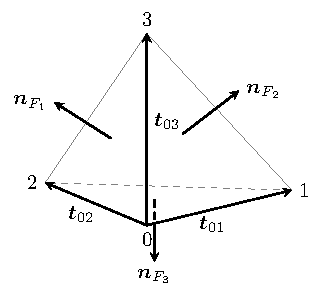
\includegraphics[width=5.0cm]{figures/Tbasis.pdf}
\end{minipage}}%%
\subfigure[Basis $\{\bs n_{F_2}, \bs n_{F_3}\}$ and $\{ \bs n^{\{0,1\}}_{\{0,1,2\}}, \bs n^{\{0,1\}}_{\{0,1,3\}}\}.$]
{\begin{minipage}[t]{0.5\linewidth}
\centering
\includegraphics*[width=5.3cm]{figures/Tedgebasis.pdf}
\end{minipage}}
\caption{Face normal basis and tangential normal basis of a vertex and an edge in a tetrahedron.}
\label{fig:normalbasis}
\end{figure}

%\begin{figure}[htbp]
%\begin{center}
%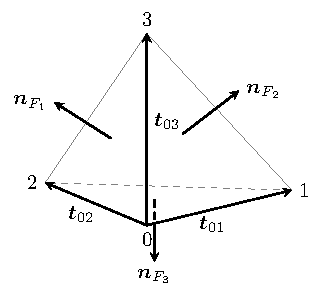
\includegraphics[width=5.05cm]{figures/Tbasis.pdf}
%\caption{Basis $\{\boldsymbol{t}_{0,1}, \boldsymbol{t}_{0,2}, \ldots, \boldsymbol{t}_{0,d}\}$ and $\{\nabla \lambda_1, \ldots, \nabla \lambda_d\}$ for $d=3$.}
%\label{fig:tnbasis}
%\end{center}
%\end{figure}

\begin{example}\rm
An important example is $f\in \Delta_0(T)$, i.e., $f$ is a vertex. Without loss of generality, let $f = \{0\}$. Then $\bs n_{f\cup\{i\}}^f$ is a unit normal vector of edge $\{0,i\}$: $\bs t_{0i}$ or $\bs t_{i0}$ depending on the orientation. Its dual basis is $\{\bs n_{F_i}/(\bs n_{F_i}\cdot \bs t_{0i}), i=1, \ldots, n\}$. See Fig.~\ref{fig:normalbasis} (a).
\end{example}


\begin{example}\rm
 Let $f = \{0,1\}$ be an edge of a tetrahedron. Then we have two bases of the normal plane $\mathscr N^f$: $\{\bs n_{F_2}, \bs n_{F_3}\}$ and $\{ \bs n^{\{0,1\}}_{\{0,1,2\}}, \bs n^{\{0,1\}}_{\{0,1,3\}}\}.$ They are dual to each other with an appropriate rescaling. See Fig.~\ref{fig:normalbasis} (b). 
\end{example}


\section{$H(\div)$ 有限元}
% The material in this section comes from \cite{BoffiBrezziFortin2013}.
% Let $\Gamma:=\partial\Omega$.
在本节中,我们考虑单纯形上$H(\div)$-协调有限元的构造。

\subsection{$H(\div)$ 空间和迹算子}
回顾 Sobolev 空间
\[
H(\div,\Omega):=\{\bs v\in L^2(\Omega;\mathbb R^d): \div\bs v\in L^2(\Omega)\}.
\]
其范数平方为 $\|\bs v\|_{\div, \Omega}^2:=\|\bs v\|_{0, \Omega}^2+\|\div\bs v\|_{0, \Omega}^2$.
\begin{lemma}
设$\bs v\in H(\div,\Omega)$,则$\bs v\cdot\bs n|_{\partial\Omega}\in H^{-1/2}(\partial\Omega)$且格林公式成立:
\[
(\div\bs v, w)_{\Omega} + (\bs v, \grad w)_{\Omega}=\langle\bs v\cdot\bs n, w\rangle_{H^{-1/2}(\partial\Omega)\times H^{1/2}(\partial\Omega)}\quad\forall~w\in H^1(\Omega).
\]
\end{lemma}

\begin{lemma}
迹算子$\bs v\in H(\div,\Omega)\to\bs v\cdot\bs n|_{\Gamma}\in H^{-1/2}(\Gamma)$是满射。
% The trace operator $\bs v\in H(\div,\Omega)\to\bs v\cdot\bs n|_{\Gamma}\in H^{-1/2}(\Gamma)$ is surjective.
\end{lemma}

% Now introduce $H(\div)$-conforming finite elements on simplexes.
% Assume $T\subset \mathbb R^d$ is a simplex with $d=2,3$. 


\subsection{Raviart-Thomas 元}

设 $T\subset \mathbb R^d$ 是 一个 $d$ 维单纯形,其中整数 $d\geq2$. Raviart-Thomas (RT) 元 \cite{RaviartThomas1977,Nedelec1980,ChenHuang2022} 的形函数空间为: $k\geq0$,
$$
V_k^{\rm RT}(T):= \mathbb P_{k}(T; \mathbb R^d) + \boldsymbol x\mathbb P_{k}(T)=\mathbb P_{k}(T; \mathbb R^d) \oplus \boldsymbol x\mathbb H_{k}(T).
$$ 
根据空间直和分解 \eqref{eq:dualPkm1vecdecomp},成立直和分解
$$
V_k^{\rm RT}(T)= (\div\mathbb P_{k+1}(T;\mathbb K))\oplus (\boldsymbol x\mathbb P_{k}(T)).
$$ 
从而,由 \eqref{eq:Hkdiv} 可得 
$$
V_k^{\rm RT}(T)\cap\ker(\div)=\mathbb P_{k}(T; \mathbb R^d)\cap\ker(\div)=\div\mathbb P_{k+1}(T;\mathbb K).
$$
自由度取为
\begin{subequations}\label{RTfemdof}
\begin{align}
(\boldsymbol v\cdot\boldsymbol  n, q)_F, & \quad q\in\mathbb P_{k}(F),  F\in\Delta_{d-1}(T),\label{RTfemdof1}\\
(\boldsymbol v, \boldsymbol q)_T, & \quad \boldsymbol q\in\mathbb P_{k-1}(T; \mathbb R^d). \label{RTfemdof2}
\end{align}
\end{subequations}

\begin{lemma}\label{lem:20250930}
设 $\boldsymbol{v}\in \mathbb P_{k}(T; \mathbb R^d)$ 满足
\begin{equation}\label{eq:20200917}
(\boldsymbol v, \boldsymbol q)_T =0 \quad \forall~\boldsymbol q\in\mathbb P_{k-1}(T; \mathbb R^d),
\end{equation}
则 $\boldsymbol v=\bs 0$。
\end{lemma}
\begin{proof}
为表述简便,记 $\Delta_{d-1}(T)$ 中的 $d+1$ 个面为 $F_i$,其中 $F_i$ 与 $T$ 的第 $i$ 个顶点相对,$\bs n_i$ 为 $F_i$ 的单位外法向量,$i=0,1,\cdots,d$。
令 $\bs t_i$ ($i=1,\ldots,d$) 表示从顶点 $0$ 指向顶点 $i$ 的单位切向量,则 $d$ 个向量 ${\bs t_1, \ldots, \bs t_d}$ 构成 $\mathbb R^d$ 的一组基(尽管它们一般不正交)。于是有
\[
\bs v=\sum_{i=1}^d\frac{\bs v\cdot\bs n_i}{\bs t_i\cdot\bs n_i}\bs t_i.
\]
由于 $\bs v\cdot\bs n_i|_{F_i}=0$,存在 $p_i\in\mathbb P_{k-1}(T)$ 使得 $\bs v\cdot\bs n_i=\lambda_ip_i$。在 \eqref{eq:20200917} 中取 $\bs q=\bs n_ip_i$ 可得
\[
(\lambda_ip_i, p_i)_T =0.
\]
因此 $p_i=0$,进而 $\boldsymbol v\cdot\bs n_i=0$,最终得到 $\boldsymbol v= 0$。
\end{proof}

\begin{lemma}\label{lem:unisovlenRTfem}
自由度 \eqref{RTfemdof} 对于形函数空间 $V_k^{\rm RT}(T)$ 是唯一可解的。
\end{lemma}
\begin{proof}
根据 $\dim\mathbb P_{k}(F)+\dim\mathbb P_{k-1}(T)=\dim\mathbb P_{k}(T)$ 和 $\dim\mathbb P_{k}(F)=\dim \mathbb H_{k}(T)$ 可知,自由度 \eqref{RTfemdof} 的总数为
\begin{equation*}
(d+1)\dim\mathbb P_{k}(F)+d\dim\mathbb P_{k-1}(T) = \dim\mathbb P_{k}(F)+d\dim\mathbb P_{k}(T) = \dim V_k^{\rm RT}(T).
\end{equation*}

设 $\boldsymbol{v}\in V_k^{\rm RT}(T)$ 满足所有自由度 \eqref{RTfemdof} 取值为零。利用分部积分及自由度 \eqref{RTfemdof} 的零值条件,可得 $(\boldsymbol{v}\cdot\boldsymbol{n})|_{\partial T}=0$,且 
\begin{equation*}
(\div\boldsymbol{v}, q)_T=(\boldsymbol{v}\cdot\boldsymbol{n},q)_{\partial T} - (\boldsymbol{v},\grad q)_T=0\quad\forall~q\in \mathbb P_{k}(T).
\end{equation*}
因此 $\div\boldsymbol{v}=0$,进而 $\boldsymbol{v}\in \mathbb P_{k}(T; \mathbb R^d)$。
再应用引理~\ref{lem:20250930},由自由度 \eqref{RTfemdof2} 为零即得 $\boldsymbol{v}=0$。
\end{proof}

根据空间分解 \eqref{eq:Pkm1vecdecomp},自由度 \eqref{RTfemdof} 可等价地改写为
\begin{subequations}\label{RTfemanotherdof}
\begin{align}
(\boldsymbol v\cdot\boldsymbol  n, q)_F, & \quad q\in\mathbb P_{k}(F),  F\in\Delta_{d-1}(T),\label{RTfemanotherdof1}\\
(\div\boldsymbol v, q)_T, & \quad q\in\mathbb P_{k}(T)/\mathbb R, \label{RTfemanotherdof2}\\
(\boldsymbol v, \boldsymbol q)_T, & \quad \boldsymbol q\in\mathbb P_{k-2}(T;\mathbb K)\boldsymbol x. \label{RTfemanotherdof3}
\end{align}
\end{subequations} 
自由度 \eqref{RTfemanotherdof} 阐明了有限元的一般构造思路:边界自由度 \eqref{RTfemanotherdof1} 由 Sobolev 空间的迹决定,确保 $H(\div)$-协调性;内部自由度 \eqref{RTfemanotherdof2} 对应散度算子的像空间,体现微分复形结构;内部自由度 \eqref{RTfemanotherdof3} 对应泡函数空间或多项式空间的直和分解。基于微分复形与 Sobolev 空间迹的这一构造方法,同样可推广至其他 Sobolev 空间的有限元设计,详见文献 \cite{ChenHuang2022}。

最低次 RT 元 ($k=0$) 的基函数为 \cite[Section 2.6]{BoffiBrezziFortin2013}
$$
\phi_i=(\boldsymbol{n}_{F_i}\cdot\nabla\lambda_i)(\texttt{v}_i-\boldsymbol{x}),\quad i=0,1,\ldots,d,
$$
其中 $\boldsymbol{n}_{F_i}$ 是 $(d-1)$ 维面 $F_i$ 的单位法向量,仅依赖于面 $F_i$,不依赖于所属的单纯形。

任意次 RT 元的基函数可参见文献 \cite[Section 9, Tables 9.1-9.2]{ArnoldFalkWinther2009}。
事实上,任意维、任意次 RT 元具有如下几何分解(参见 \cite{ArnoldFalkWinther2009})
$$
\mathbb P_k(T;\mathbb R^d)+\mathbb P_k(T)\bs x=\Oplus_{i=0}^d\mathbb P_{k}(F_{i})(\texttt{v}_i-\boldsymbol{x}) \oplus \Oplus_{i=1}^d\lambda_i\mathbb P_{k-1}(T)(\texttt{v}_i-\boldsymbol{x}).
$$
据此几何分解,可构造出 RT 元的基函数。



\subsection{Brezzi-Douglas-Marini 元}

Brezzi-Douglas-Marini (BDM) 元 \cite{BrezziDouglasMarini1985,BrezziDouglasDuranFortin1987,Nedelec1986,ChenHuang2022,ChenChenHuangWei2024,ChenHuang2024} 的形函数空间为 $V_k^{\rm BDM}(T):= \mathbb P_{k}(T; \mathbb R^d)$,其中 $k\geq1$。
自由度取为
\begin{subequations}\label{BDMfemdof}
\begin{align}
(\boldsymbol v\cdot\boldsymbol  n, q)_F, & \quad q\in\mathbb P_{k}(F),  F\in\Delta_{d-1}(T),\label{BDMfemdof1}\\
(\boldsymbol v, \boldsymbol q)_T, & \quad \boldsymbol q\in\grad \mathbb P_{k-1}(T)\oplus\mathbb P_{k-2}(T;\mathbb K)\boldsymbol x. \label{BDMfemdof2}
\end{align}
\end{subequations}



\begin{lemma}\label{lem:unisovlenBDMfem}
自由度 \eqref{BDMfemdof} 对于形函数空间 $V_k^{\rm BDM}(T)$ 是唯一可解的。
\end{lemma}
\begin{proof}
根据空间分解 \eqref{eq:Pkm1vecdecomp}、关系式 $\dim\mathbb P_{k}(F)=\dim \mathbb H_{k}(T)$ 及 $\dim\mathbb P_{k}(F)+\dim\mathbb P_{k-1}(T)=\dim\mathbb P_{k}(T)$ 可知,自由度 \eqref{BDMfemdof} 的总数为
\begin{equation*}
(d+1)\dim\mathbb P_{k}(F)+d\dim\mathbb P_{k-1}(T) - \dim\mathbb H_{k}(T) = d\dim\mathbb P_{k}(F)+d\dim\mathbb P_{k-1}(T) = \dim V_k^{\rm BDM}(T).
\end{equation*}

设 $\boldsymbol{v}\in V_k^{\rm BDM}(T)$ 满足所有自由度 \eqref{BDMfemdof} 取值为零。利用分部积分及自由度 \eqref{BDMfemdof} 的零值条件,可得 $(\boldsymbol{v}\cdot\boldsymbol{n})|_{\partial T}=0$,且
\begin{equation*}
(\div\boldsymbol{v}, q)_T=(\boldsymbol{v}\cdot\boldsymbol{n},q)_{\partial T} - (\boldsymbol{v},\grad q)_T=0\quad\forall~q\in \mathbb P_{k-1}(T).
\end{equation*}
因此 $\div\boldsymbol{v}=0$,进而由分部积分得
\begin{equation*}
(\boldsymbol{v},\grad q)_T=0\quad\forall~q\in \mathbb P_{k}(T).
\end{equation*}
结合自由度 \eqref{BDMfemdof2} 的零值条件,可得
\begin{equation*}
(\boldsymbol v, \boldsymbol q)_T =0 \quad \forall~\boldsymbol q\in\mathbb P_{k-1}(T; \mathbb R^d).
\end{equation*}
再应用引理~\ref{lem:20250930} 即得 $\boldsymbol{v}=0$。
\end{proof}


%\newpage
接下来我们给出当 $k\geq2$ 时 $H(\div)$ 泡函数空间的显式刻画。定义多项式泡函数空间
\[
\mathbb B_k(\div, T):=\{\bs v\in\mathbb P_{k}(T;\mathbb R^d): \bs v\cdot\bs n|_{\partial K}=0\}.
\]
由 BDM 元的唯一可解性知,
\[
\dim \mathbb B_k(\div, T) = d\binom{k+d}{d} - (d+1)\binom{k+d-1}{d-1} = (k-1)\binom{k+d-1}{d-1}.
\]



\begin{lemma}
对于 $k\geq2$ 成立
\begin{equation}\label{eq:Hdivbubbleidentity}
\mathbb B_k(\div, T)=\sum_{0\leq i<j\leq d}\lambda_i\lambda_j\mathbb P_{k-2}(T)\bs t_{i,j},
\end{equation}
其中 $\bs t_{i,j}:=\textnormal{\texttt{v}}_j-\textnormal{\texttt{v}}_i$,$\textnormal{\texttt{v}}_0, \textnormal{\texttt{v}}_1, \cdots, \textnormal{\texttt{v}}_d$ 是单纯形 $T$ 的顶点。
\end{lemma}
\begin{proof}
验证 $\lambda_i\lambda_j\mathbb P_{k-2}(T)\boldsymbol t_{i,j}\subseteq \mathbb B_k(\div, T)$ 的依据是以下事实:
$$\lambda_i\lambda_j \boldsymbol t_{i,j}\cdot \boldsymbol n_{\ell}|_{F_{\ell}} = 0, \quad \ell = 0, 1, \cdots, d.$$
事实上,若 $\ell = i$ 或 $\ell = j$,则 $\lambda_i\lambda_j|_{F_{\ell}} =0$;否则 $\boldsymbol t_{i,j}\cdot \boldsymbol n_{\ell} = 0$。接下来证明 $\mathbb B_k(\div, T)$ 中的每个函数均可表示为 $\lambda_i\lambda_j \boldsymbol t_{i,j}$ 的线性组合。


任取 $\bs v\in\mathbb B_k(\div, T)$。由于 $\{\bs t_{0,1}, \ldots, \bs t_{0,d}\}$ 构成 $\mathbb R^d$ 的一组基,故 $\bs v$ 可表示为
$$\bs v=p_1\bs t_{0,1}+\cdots+p_d\bs t_{0,d},$$ 
其中 $p_1, \ldots, p_d\in\mathbb P_k(T)$。注意到 $\bs v\cdot\bs n|_{\partial T}=0$,因此
\[
p_i\bs t_{0,i}\cdot\bs n_i|_{F_i}=0 \quad (i=1,\ldots,d).
\]
由此可知 $p_i|_{F_i} = 0$  对 $i=1,\dots,d$ 成立,于是可以令
\[
\boldsymbol v = \sum_{i=1}^{d} \lambda_i q_i \boldsymbol t_{0,i}, \quad q_i\in \mathbb P_{k-1}(T).
\]
进一步将 $q_i$ 展开为
\[
q_i = \lambda_0 q_0 + \sum_{j=1}^{d} \lambda_j q_{ij},
\]
其中
\[
q_0 \in \mathbb P_{k-2}(T), \quad q_{ij} \in \sum_{\alpha_j+\cdots+\alpha_{d}=k-2 \atop \alpha_j,\cdots,\alpha_{d}\in\mathbb N} \mathrm{span}\{\lambda_j^{\alpha_j}\cdots \lambda_d^{\alpha_d}\},
\]
并且 $q_{ij}$ 的表达中不包含 $\lambda_0, \lambda_1, \ldots, \lambda_{j-1}$。

由 $\boldsymbol n\cdot \boldsymbol v|_{F_0}=0$ 且 $\boldsymbol t_{0,i}\cdot \boldsymbol n_0\neq0$,可得
\[
\sum_{i=1}^{d} \lambda_i q_i|_{F_0} = 0,
\quad
\textrm{ 即 }
\quad
\sum_{i=1}^{d}\sum_{j=1}^{d}(\lambda_i \lambda_j q_{ij})|_{F_0} = 0 \quad\Leftrightarrow\quad \sum_{i=1}^{d}\sum_{j=1}^{d}\lambda_i \lambda_j q_{ij} = 0.
\]
由于 $q_{ij}$ 的表达中不含 $\lambda_0, \lambda_1, \ldots, \lambda_{j-1}$,利用数学归纳法可证
\[
\sum_{i=\ell}^{d}\sum_{j=\ell}^{d}\lambda_i \lambda_j q_{ij} = 0,\quad \ell=1,\dots,d.
\]
可进一步得到
\[
\sum_{j=i}^{d} \lambda_j q_{ij} + \sum_{j=i+1}^{d} \lambda_j q_{ji} = 0, \quad i=1,\dots,d.
\]
由此可得
\begin{align*}
\sum_{i=1}^{d}\sum_{j=i}^{d} \lambda_i \lambda_j q_{ij} \boldsymbol t_{0,i}
&= - \sum_{i=1}^{d-1}\sum_{j=i+1}^{d} \lambda_i \lambda_j q_{ji} \boldsymbol t_{0,i}
= - \sum_{j=1}^{d-1}\sum_{i=j+1}^{d} \lambda_i \lambda_j q_{ij} \boldsymbol t_{0,j} 
= - \sum_{i=2}^{d}\sum_{j=1}^{i-1} \lambda_i \lambda_j q_{ij} \boldsymbol t_{0,j}.
\end{align*}
因此
\begin{align*}
\boldsymbol v&=\sum_{i=1}^{d}\lambda_i q_i\boldsymbol t_{0,i} = \sum_{i=1}^{d}\lambda_i \lambda_{0}q_{0}\boldsymbol t_{0,i} + \sum_{i=1}^{d}\sum_{j=1}^{d}\lambda_i\lambda_jq_{ij}\boldsymbol t_{0,i} \\
&= \sum_{i=1}^{d}\lambda_i \lambda_{0}q_{0}\boldsymbol t_{0,i}
+ \sum_{i=2}^{d}\sum_{j=1}^{i-1}\lambda_i\lambda_jq_{ij}\boldsymbol t_{0,i} + \sum_{i=1}^{d}\sum_{j=i}^{d}\lambda_i\lambda_jq_{ij}\boldsymbol t_{0,i} \\
&= \sum_{i=1}^{d}\lambda_i \lambda_{0}q_{0}\boldsymbol t_{0,i}
+ \sum_{i=2}^{d}\sum_{j=1}^{i-1}\lambda_i\lambda_jq_{ij}\boldsymbol t_{0,i} -\sum_{i=2}^{d}\sum_{j=1}^{i-1}\lambda_i\lambda_jq_{ij}\boldsymbol t_{0,j} \\
&= \sum_{i=1}^{d}\lambda_i \lambda_{0}q_{0}\boldsymbol t_{0,i}
+ \sum_{i=2}^{d}\sum_{j=1}^{i-1}\lambda_i\lambda_jq_{ij}\boldsymbol t_{j,i},
\end{align*}
得证。
\end{proof}


最低次 BDM 元 ($k=1$) 的基函数为 \cite[Section 2.6]{BoffiBrezziFortin2013}
$$
\phi_{\ell,i}=(\boldsymbol{n}_{F_{\ell}}\cdot\nabla\lambda_{\ell})\lambda_i\boldsymbol{t}_{i,\ell},\quad 0\leq \ell \leq d,\; 0\leq i\neq \ell \leq d.
$$
任意次 BDM 元的基函数可参见文献 \cite[Section 9, Table 9.1, Table 9.4]{ArnoldFalkWinther2009}。

文献 \cite{ArnoldFalkWinther2009} 中 BDM 元基函数还比较复杂,但它们都可以通过切向法向分解来构造。


\textcolor{red}{引出切向法向分解 BDM元的构造基函数。}







\section{$H(\curl)$ 有限元}

Assume $d=3$.
Define
\[
H(\curl,\Omega):=\{\bs v\in L^2(\Omega;\mathbb R^3): \curl\bs v\in L^2(\Omega;\mathbb R^3)\}.
\]
with squared  norm $\|\bs v\|_{\curl, \Omega}^2:=\|\bs v\|_{0, \Omega}^2+\|\curl\bs v\|_{0, \Omega}^2$.

The results on the trace of $H(\curl,\Omega)$ can be found in \cite{BuffaCostabelSheen2002,BuffaCiarlet2001,BuffaCiarlet2001a}.
 For any regular vector field $\bs v$ in $\Omega$, we define the tangential trace $\gamma_{t}(\bs v):=\bs n\times \bs v|_{\Gamma}$, and the projection on the tangential plane $\pi_{t}(\bs v):=\bs n\times\bs v\times  \bs n|_{\Gamma}$. Let
 \[
 \bs H^{-1/2}(\div_{\Gamma}, \Gamma):=\{\bs\lambda\in V_{\pi}': \div_{\Gamma}\bs\lambda\in H^{-1/2}(\Gamma)\},
 \]
 \[
 \bs H^{-1/2}(\curl_{\Gamma}, \Gamma):=\{\bs\lambda\in V_{\gamma}': \curl_{\Gamma}\bs\lambda\in H^{-1/2}(\Gamma)\},
 \]
 where $V_{\gamma}:=\gamma_{t}(\bs H^{1/2}(\Gamma))$ and $V_{\pi}:=\pi_{t}(\bs H^{1/2}(\Gamma))$.
Spaces $ \bs H^{-1/2}(\div_{\Gamma}, \Gamma)$ and $ \bs H^{-1/2}(\curl_{\Gamma}, \Gamma)$ are dual to each other with the pivot space $L_t^2(\Gamma):=\{\bs \lambda\in L^2(\Gamma;\mathbb R^3): \bs \lambda\cdot\bs n=0\}$.

If the surface $\Gamma$ was regular, then
\[
V_{\gamma}=V_{\pi}=\{\bs\lambda\in\bs H^{1/2}(\Gamma, \mathbb R^3): \bs\lambda\cdot\bs n=0\}.
\]
In the case of piecewise regular surfaces, the spaces $V_{\gamma}$ and $V_{\pi}$ are different (see \cite{BuffaCiarlet2001}).

\begin{lemma}
The trace operators $\gamma_{t}:  H(\curl,\Omega)\to\bs H^{-1/2}(\div_{\Gamma}, \Gamma)$ and $\pi_{t}:  H(\curl,\Omega)\to\bs H^{-1/2}(\curl_{\Gamma}, \Gamma)$ are linear, continuous and surjective. And we have the 
Green's formula
\[
(\curl\bs v, \bs\phi)_{\Omega} - (\bs v, \curl\bs\phi)_{\Omega}=\langle\gamma_t\bs v, \pi_t\bs \phi\rangle\quad\forall~\bs v, \bs \phi\in H(\curl,\Omega).
\]
\end{lemma}

Now introduce $H(\curl)$-conforming finite elements on tetrahedrons.
Assume $K\subset \mathbb R^3$ is a tetrahedron.
Thanks to \eqref{eq:vector3polyspacedecomp1}, define the shape function space
\[
V_{k,\ell}^c(K):=\grad\mathbb P_{k+1}(K)\oplus \boldsymbol x\times\mathbb P_{\ell-1}(K; \mathbb R^3)=\mathbb P_{k}(K; \mathbb R^3) + \boldsymbol x\times\mathbb P_{\ell-1}(K; \mathbb R^3),
\]
where $\ell=k, k+1$ for $k\geq1$, and $\ell=1$ for $k=0$. 
The degrees of freedom $\mathcal N_{k,\ell}^c(K)$ are given by
\begin{align}
(\boldsymbol v\cdot\boldsymbol t, q)_e & \quad\forall~q\in\mathbb P_{k}(e),  e\in\mathcal E(K),\label{Hcurlfem3ddof1}\\
(\boldsymbol n\times\boldsymbol v\times\boldsymbol  n, \bs q)_F & \quad\forall~q\in\curl_F\mathbb P_{
\ell-1}(F)\oplus\bs x\mathbb P_{k-2}(F),  F\in\mathcal F(K),\label{Hcurlfem3ddof2}\\
(\boldsymbol v, \boldsymbol q)_K & \quad\forall~\boldsymbol q\in\curl\mathbb P_{\ell-2}(K; \mathbb R^3)\oplus\boldsymbol x\mathbb P_{k-3}(K). \label{Hcurlfem3ddof3}
\end{align}
Since $\ell=k, k+1$, we have $\curl_F\mathbb P_{
\ell-1}(F)\oplus\bs x\mathbb P_{k-2}(F)=\mathbb P_{
\ell-2}(F;\mathbb R^2)+\bs x\mathbb P_{k-2}(F)$ and $\curl\mathbb P_{\ell-2}(K; \mathbb R^3)\oplus\boldsymbol x\mathbb P_{k-3}(K)=\mathbb P_{
\ell-3}(F;\mathbb R^3)+\boldsymbol x\mathbb P_{k-3}(K)$.

Apparently $\bs v\cdot \bs t|_e\in\mathbb P_{k}(e)$ for any $\bs v\in V_{k,\ell}^c(K)$ and $e\in\mathcal E(K)$.
And $\curl V_{k,\ell}^c(K)=\curl\mathbb P_{\ell}(K;\mathbb R^3)$.




\begin{lemma}\label{lem:unisovlenHdivfem}
The finite element triple $(K, V_{k,\ell}^c(K), \mathcal N_{k,\ell}^c(K))$ is well-defined.
\end{lemma}
\begin{proof}
It is easy to check that the number of the degrees of freedom \eqref{Hcurlfem3ddof1}-\eqref{Hcurlfem3ddof3}  is equal to $\dim V_{k,\ell}^c(K)$.


Take any $\boldsymbol v\in V_{k,\ell}^c(K)$ and
suppose all the degrees of freedom \eqref{Hcurlfem3ddof1}-\eqref{Hcurlfem3ddof3} vanish. 
By the vanishing degrees of freedom \eqref{Hcurlfem3ddof1}-\eqref{Hcurlfem3ddof2}, we get $\bs v\in H_0(\curl, K)$. 
Now consider $\curl\bs v\in H_0(\div, K)\cap\cap \mathbb P_{\ell-1}(K;\mathbb R^3)$.
By the vanishing degrees of freedom \eqref{Hcurlfem3ddof3}, we get 
\[
(\curl\boldsymbol v, \boldsymbol q)_K = \quad\forall~\boldsymbol q\in\mathbb P_{\ell-2}(K; \mathbb R^3).
\]
Then by the well-posedness of the finite element triple $(K, V_{\ell-1,\ell-1}^d(K), \mathcal N_{\ell-1,\ell-1}^d(K))$, we obtain $\curl\boldsymbol v=0$. Hence $\boldsymbol v\in \grad\mathbb P_{k+1}(K)\cap H_0(\curl, K)$. Then there exists $w\in\mathbb P_{k-3}(K)$ such that $\bs v=\nabla(b_Kw)$, where $b_K:=\lambda_1\lambda_2\lambda_3\lambda_4$ is the bubble function.
It follows from the vanishing degrees of freedom \eqref{Hcurlfem3ddof3} that
\[
(b_Kw, \div\boldsymbol q)_K = \quad\forall~\boldsymbol q\in\boldsymbol x\mathbb P_{k-3}(K).
\]
Due to \eqref{eq:vector3polyspacedecomp2},  it holds $\div(\boldsymbol x\mathbb P_{k-3}(K))=\mathbb P_{k-3}(K)$. As a result, $w=0$ and then $\boldsymbol v=\bs 0$.
\end{proof}

We can see that the finite element triple $(K, V_{k,k+1}^c(K), \mathcal N_{k,k+1}^c(K))$ is the first kind N\'ed\'elec element \cite{Nedelec1980}, and $(K, V_{k,k}^c(K), \mathcal N_{k,k}^c(K))$ is the second kind N\'ed\'elec  element \cite{Nedelec1986}.

Next we present the explicit expression of the $H(\curl)$ bubble functions for $k\geq3$. Let
\[
\mathring V_{k}^c(K):=\{\bs v\in\mathbb P_{k}(K;\mathbb R^3): \bs v\times\bs n|_{\partial K}=0\},\quad
V_{k,b}^c(K):=\sum_{i=1}^4b_{F_i}\mathbb P_{k-3}(K)\nabla\lambda_{i}.
\]
\begin{lemma}
It holds for $k\geq3$ that
\begin{equation}\label{eq:Hcurlbubbleidentity}
\mathring V_{k}^c(K)=V_{k,b}^c(K).
\end{equation}
\end{lemma}
\begin{proof}
It is easy to see that $V_{k,b}^c(K)\subseteq\mathring V_{k}^c(K)$. Next let's prove $\mathring V_{k}^c(K)\subseteq V_{k,b}^c(K)$. Take any $\bs v\in\mathring V_{k}^c(K)$. Since $\{\nabla\lambda_{1}, \nabla\lambda_{2}, \nabla\lambda_{3}\}$ forms a basis of $\mathbb R^3$, we can express 
$$\bs v=q_1\nabla\lambda_{1}+q_2\nabla\lambda_{2}+q_3\nabla\lambda_{3},$$ 
where $q_1, q_2, q_3\in\mathbb P_k(K)$. Noting that $\bs v\times\bs n|_{\partial K}=0$, we get
\[
(q_2\nabla\lambda_{2}\times\bs n_1+q_3\nabla\lambda_{3}\times\bs n_1)|_{F_1}= 
(q_1\nabla\lambda_{1}\times\bs n_2+q_3\nabla\lambda_{3}\times\bs n_2)|_{F_2}= 
(q_1\nabla\lambda_{1}\times\bs n_3+q_2\nabla\lambda_{2}\times\bs n_3)|_{F_3}=0,
\]
\begin{equation}\label{eq:20201002-3}
(q_1\nabla\lambda_{1}\times\bs n_4+q_2\nabla\lambda_{2}\times\bs n_4+q_3\nabla\lambda_{3}\times\bs n_4)|_{F_4}=0.
\end{equation}
Hence $\lambda_2\lambda_3|q_1$, $\lambda_1\lambda_3|q_2$ and $\lambda_1\lambda_2|q_3$. This means
there exist $\tilde q_1, \tilde q_2, \tilde q_3\in\mathbb P_{k-2}(K)$ such that $q_1=\tilde q_1\lambda_2\lambda_3$, $q_2=\tilde q_2\lambda_1\lambda_3$ and $q_3=\tilde q_3\lambda_1\lambda_2$.  %Then
%\[
%\bs v=\tilde q_1\lambda_2\lambda_3\nabla\lambda_{1}+\tilde q_2\lambda_1\lambda_3\nabla\lambda_{2}+\tilde q_3\lambda_1\lambda_2\nabla\lambda_{3}.
%\]
Since $\nabla\lambda_{1}\times\bs n_4+\nabla\lambda_{2}\times\bs n_4+\nabla\lambda_{3}\times\bs n_4=\bs0$,
it follows from~\eqref{eq:20201002-3} that
\[
((q_1-q_3)\nabla\lambda_{1}\times\bs n_4+(q_2-q_3)\nabla\lambda_{2}\times\bs n_4)|_{F_4}=0.
\]
Consequently $\lambda_4|(\tilde q_1\lambda_3-\tilde q_3\lambda_1)$ and $\lambda_4|(\tilde q_2\lambda_3-\tilde q_3\lambda_2)$. 
Thus there exist $p_{ij}\in\mathbb P_{k-3}(K)$ ($i=1,2,3, j=1,2$) such that
\[
\tilde q_1=\lambda_1p_{11}+\lambda_4p_{12},
\quad \tilde q_2=\lambda_2p_{21}+\lambda_4p_{22}, \quad \tilde q_3=\lambda_3p_{31}+\lambda_4p_{32}.
\]
Moreover we have $\lambda_4|(p_{11}-p_{31})$ and $\lambda_4|(p_{21}-p_{31})$.
Therefore we acquire from $\nabla\lambda_{3}=-\nabla\lambda_{1}-\nabla\lambda_{2}-\nabla\lambda_{4}$ that
\begin{align*}
\bs v&=\tilde q_1\lambda_2\lambda_3\nabla\lambda_{1}+\tilde q_2\lambda_1\lambda_3\nabla\lambda_{2}+\tilde q_3\lambda_1\lambda_2\nabla\lambda_{3} \\
&=b_{F_4}(p_{11}\nabla\lambda_{1}+p_{21}\nabla\lambda_{2}+p_{31}\nabla\lambda_{3}) +p_{12}b_{F_1}\nabla\lambda_{1}+p_{22}b_{F_2}\nabla\lambda_{2}+p_{32}b_{F_3}\nabla\lambda_{3} \\
&=b_{F_4}((p_{11}-p_{31})\nabla\lambda_{1}+(p_{21}-p_{31})\nabla\lambda_{2}) - p_{31}b_{F_4}\nabla\lambda_{4} +p_{12}b_{F_1}\nabla\lambda_{1}+p_{22}b_{F_2}\nabla\lambda_{2}+p_{32}b_{F_3}\nabla\lambda_{3},
\end{align*}
which ends the proof.
\end{proof}

We have from \eqref{eq:Hcurlbubbleidentity} that
\begin{align*}
\dim\mathring V_{k}^c(K)=4\dim\mathbb P_{k-3}(K)-\dim\mathbb P_{k-4}(K)=\frac{1}{2}(k^2-1)(k-2).
\end{align*}
We can also acquire $\dim\mathring V_{k}^c(K)$ from the unisolvence of the second kind N\'ed\'elec element.

\section{有限元 de Rham 复形}
Recall that a Hilbert complex is a sequence of Hilbert spaces connected by a sequence of linear operators satisfying the property: the composition of two consecutive operators is vanished. A Hilbert complex is exact means the range of each map is the kernel of the succeeding map. As $\Omega$ is topologically trivial, the following de Rham Complex of $\Omega$ is exact
\begin{equation}\label{eq:derham}
0\xrightarrow{} H^1(\Omega)\xrightarrow{\grad}\boldsymbol H(\curl;\Omega)\xrightarrow{\curl}\boldsymbol H(\div;\Omega)\xrightarrow{\div}L^2(\Omega) \xrightarrow{}0.
\end{equation}

给出泡函数复形。